\makeatletter
\@ifundefined{bwtrue}{\newif\ifbw\bwfalse}{}
\@ifundefined{acmtrue}{\newif\ifacm\acmtrue}{}
\makeatother
\makeatletter
\let\@period=\,
\makeatother
\documentclass[a4paper]{article}
\usepackage{xspace}
\usepackage{color}
\usepackage[leqno]{amsmath}
\usepackage{amssymb}
\usepackage{array}
\usepackage{tabularx}
\usepackage{booktabs}
\usepackage{url}
\usepackage{hyperref}
\usepackage{breakurl}
\usepackage{graphicx}
%\usepackage{rotating}
%\usepackage{adjustbox}
\usepackage{lscape}
\usepackage{subfig}
\usepackage{epsfig}
\usepackage{multicol}
\usepackage{float}
\usepackage[final]{fixme}
\newif\ifcomments
\commentsfalse
\usepackage{url}
\makeatletter
\def\url@leostyle{%
  \@ifundefined{selectfont}{\def\UrlFont{\small\sf}}{\def\UrlFont{\small\sf}}}
\makeatother
\urlstyle{leo}
\usepackage[normalem]{ulem}
\usepackage{xspace}
%same notation policy for each instance of figure, thm, etc
\newcommand{\myfig}{Fig.~}
\newcommand{\mytab}{Tab.~}
\newcommand{\mysec}{Sec.~}
\newcommand{\mychap}{Chap.~}
\newcommand{\myapp}{App.~}
\newcommand{\etal}{et~al.\xspace}
\newcommand{\wrt}{w.r.t.\xspace}
\newcommand{\eg}{e.g.\xspace}
\newcommand{\ie}{i.e.\xspace}
\newcommand{\etc}{etc.\xspace}
\newcommand{\cf}{see\xspace}

%les maths comme au lycee
\let\eset\emptyset
\newcommand{\rplus}[1]{\mathop{{#1}^{+}}}
\newcommand{\rstar}[1]{\mathop{{#1}^{*}}}
\newcommand{\transc}[1]{\mathop{{#1}^{+}}}
\newcommand{\maybe}[1]{\mathop{{#1}^{?}}}

%def
  \newcommand{\dfnshort}[2]{{#1}\triangleq{#2}}
  \newcommand{\dfn}[2]{{#1}~\triangleq~{#2}}

%sets
\newcommand{\setcal}[1]{\mathcal{#1} }
\newcommand{\setbf}[1]{\mathbb{#1} }
\newcommand{\setfrak}[1]{\mathfrak{#1} }


  %writes, reads, barriers
  \let\setset\setbf
  \newcommand{\evts}{\setset{E}}

  \newcommand{\lwf}{\textsf{fence}}
  \newcommand{\mfence}{\ensuremath{\mathsf{mfence}}}
  \newcommand{\lwfence}{\ensuremath{\mathsf{fence}}}
  \newcommand{\ff}{\textsf{fence.sc}}
  \newcommand{\ffence}{\ensuremath{\mathsf{f{\kern-0.1em}fence}}}
  \newcommand{\fences}{\ensuremath{\mathsf{fence}}}
  \newcommand{\relw}{\ensuremath{\mathsf{rel}}}
  \newcommand{\acqr}{\ensuremath{\mathsf{acq}}}
  \newcommand{\cumul}{\ensuremath{\mathsf{cumul}}}
  \newcommand{\Acumul}{\ensuremath{\mathsf{A{\kern-0.3em}-{\kern-0.3em}cumul}}}

  %procs
  \newcommand{\pr}{\operatorname{proc}}

  %locs
  \newcommand{\lo}{\ell}
  \newcommand{\loc}{\operatorname{addr}}

  %vals 
  \newcommand{\val}{\operatorname{val}}

%relations
\newcommand{\stacklabel}[1]
%{\stackrel{\smash{\scriptscriptstyle\#1}}}
{\stackrel{\smash{\scriptstyle\textnormal{#1}}}}
  %any
  \newcommand{\rln}[1]{\ensuremath{\xrightarrow{#1}}}

  %po
  \newcommand{\iico}{\ensuremath{\mathsf{ii}}}
  \newcommand{\ctrlcfence}{\ensuremath{\mathsf{ctrlcfence}}}
  \newcommand{\ctrl}{\ensuremath{\mathsf{ctrl}}}
  \newcommand{\data}{\ensuremath{\mathsf{data}}}
  \newcommand{\addr}{\ensuremath{\mathsf{addr}}}
  \newcommand{\ddreg}{\ensuremath{\mathsf{dd}}}
  \newcommand{\rfreg}{{\mathsf{rfreg}}}
  \newcommand{\isb}{\ensuremath{\mathsf{isb}}}
  \newcommand{\isync}{\ensuremath{\mathsf{isync}}}
  \newcommand{\po}{\ensuremath{\mathsf{po}}}
  \newcommand{\ppo}{\ensuremath{\mathsf{ppo}}}
  %rf
  \newcommand{\rf}{\ensuremath{\mathsf{rf}}}
  %rfe
  \newcommand{\rfe}{\ensuremath{\mathsf{rfe}}}
  %rfi
  \newcommand{\rfi}{\ensuremath{\mathsf{rfi}}}
  %co
  \newcommand{\co}{\ensuremath{\mathsf{co}}}
  \newcommand{\coi}{\ensuremath{\mathsf{coi}}}
  \newcommand{\ews}{\ensuremath{\mathsf{coe}}}
  %fr
  \newcommand{\fr}{\ensuremath{\mathsf{fr}}}
  \newcommand{\ifr}{\ensuremath{\mathsf{fri}}}
  \newcommand{\efr}{\ensuremath{\mathsf{fre}}}
  %hb
  \newcommand{\com}{\ensuremath{\mathsf{com}}}
  \newcommand{\cause}{\ensuremath{\mathsf{cause}}}
  \newcommand{\hb}{\ensuremath{\mathsf{hb}}}
\newcommand{\propbase}{\operatorname{\ensuremath{\mathsf{prop{\kern-0.00em}-{\kern-0.1em}base}}}}
\newcommand{\prop}{\operatorname{\ensuremath{\mathsf{prop}}}}
  %poloc
  \newcommand{\polocllh}{\operatorname{\ensuremath{\mathsf{po{\kern-0.00em}-{\kern-0.1em}loc{\kern-0.00em}-{\kern-0.05em}llh}}}}
  \newcommand{\poloc}{\operatorname{\ensuremath{\mathsf{po{\kern-0.00em}-{\kern-0.05em}loc}}}}
  %criteria
  \newcommand{\acyclic}{\operatorname{acyclic}}
  \newcommand{\reflexive}{\operatorname{reflexive}}
  \newcommand{\irrefl}{\operatorname{irreflexive}}
  %po restricted to some events
  \newcommand{\WW}{\operatorname{\ensuremath{\mathsf{{WW}}}}}
  \newcommand{\RM}{\operatorname{\ensuremath{\mathsf{RM}}}}
  \newcommand{\RW}{\operatorname{\ensuremath{\mathsf{RW}}}}
  \newcommand{\RR}{\operatorname{\ensuremath{\mathsf{RR}}}}
  \newcommand{\RB}{\operatorname{\ensuremath{\mathsf{RB}}}}
  \newcommand{\MW}{\operatorname{MW}}
  \newcommand{\WM}{\operatorname{WM}}
  \newcommand{\WR}{\operatorname{\ensuremath{\mathsf{WR}}}}

\newcommand{\wide}{wide}
\newcommand{\wider}{wider}
\newcommand{\widest}{widest}
\newcommand{\narrow}{narrow}
\renewcommand{\narrower}{narrower}
\newcommand{\narrowest}{narrowest}
\newcommand{\narrowerop}{\operatorname{narrower}}

%%%Litmus
%%basic format
\let\prog\textsf
\let\as\texttt
\let\ltest\textbf

%% Conventional processor
\newcommand{\proc}[1]{\ensuremath{P_{#1}}}
%% Format graphs in columns
\makeatletter
\@ifundefined{useepstrue}{\newif\ifuseeps\useepsfalse}{}
\makeatother
\newlength{\fmtlength}
\ifuseeps
\newcommand{\fmtgraphcol}[3]
{\setlength{\fmtlength}{\linewidth}%
\addtolength{\fmtlength}{-#2}%
\framebox{\resizebox{\fmtlength}{#3}{\includegraphics{#1.eps}}}}
\else
\newcommand{\fmtgraphcol}[3]
{\setlength{\fmtlength}{\linewidth}%
\addtolength{\fmtlength}{-#2}%
\framebox{\resizebox{\fmtlength}{#3}{\input{#1.pstex_t}}}}
\fi
%%Format graph explicit width
\ifuseeps
\newcommand{\fmtgraph}[3]
{\resizebox{#2}{#3}{\includegraphics{#1.eps}}}
\newcommand{\tfmtgraph}[1]{\framebox{\includegraphics{#1.eps}}}
\else
\newcommand{\fmtgraph}[3]
{\resizebox{#2}{#3}{\input{#1.pstex_t}}}
\newcommand{\tfmtgraph}[1]{\framebox{\input{#1.pstex_t}}}
\fi
%%%%Test for figures as in the tutorial
% fix up fig2dev fonts to make actions in \sf
\iftrue
\makeatletter
% for the fig2dev version on P laptop
\gdef\SetFigFontNFSS#1#2#3#4#5{%
  \reset@font\fontsize{#1}{#2pt}%
%  \fontfamily{#3}\fontseries{#4}\fontshape{#5}%
  \fontfamily{\sfdefault}\fontseries{#4}\fontshape{#5}%
  \selectfont}%
% for the fig2dev version on P desktop
\gdef\SetFigFont#1#2#3#4#5{%
  \reset@font\fontsize{#1}{#2pt}%
%  \fontfamily{#3}\fontseries{#4}\fontshape{#5}%
  \fontfamily{\sfdefault}\fontseries{#4}\fontshape{#5}%
  \selectfont}
\makeatother
\newcommand{\asm}[1]{\texttt{#1}}
\newcommand{\myth}[1]{\ensuremath{\mathsf{T}_#1}}
\newcommand{\mylegend}[2]{#1}
\ifbw\newcommand{\bw}{-bw}\else\newcommand{\bw}{}\fi
\ifuseeps
\newcommand{\locfmt}[1]{\includegraphics{#1.eps}}
\newcommand{\newfmt}[1]{\includegraphics{img/#1.eps}}
\newcommand{\insfmt}[1]{\scalebox{0.28}{\includegraphics{ins/#1.eps}}}
\else
\newcommand{\locfmt}[1]{\input{#1.pstex_t}}
\newcommand{\newfmt}[1]{\input{img/#1\bw.pstex_t}}
\newcommand{\insfmt}[1]{\scalebox{0.28}{\input{ins/#1\bw.pstex_t}}}
\fi
\fi

\newcommand{\NEW}[1]{\textcolor{blue}{#1}}

\newcolumntype{Y}{@{}r@{\,}X}
%%Decorate instruction with a label
\newcommand{\instab}[2]{\ \(#2\)  & \as{#1}}
%%Pseudo-code load & store
\newcommand{\pset}[2]{\(\as{#1} \leftarrow \as{#2}\)}
\newcommand{\pstore}[2]{\pset{#2}{#1}}
\newcommand{\pload}[2]{\pset{#1}{#2}}
%%trick to add vertical space somewhere
\newcommand{\haut}{\rule{0ex}{2ex}}
\newcommand{\bas}{\rule[-1ex]{0.5ex}{0ex}}


\usepackage{xspace}
%same notation policy for each instance of figure, thm, etc
\newcommand{\myfig}{Fig.~}
\newcommand{\mytab}{Tab.~}
\newcommand{\mysec}{Sec.~}
\newcommand{\mychap}{Chap.~}
\newcommand{\myapp}{App.~}
\newcommand{\etal}{et~al.\xspace}
\newcommand{\wrt}{w.r.t.\xspace}
\newcommand{\eg}{e.g.\xspace}
\newcommand{\ie}{i.e.\xspace}
\newcommand{\etc}{etc.\xspace}
\newcommand{\cf}{see\xspace}

%les maths comme au lycee
\let\eset\emptyset
\newcommand{\rplus}[1]{\mathop{{#1}^{+}}}
\newcommand{\rstar}[1]{\mathop{{#1}^{*}}}
\newcommand{\transc}[1]{\mathop{{#1}^{+}}}
\newcommand{\maybe}[1]{\mathop{{#1}^{?}}}

%def
  \newcommand{\dfnshort}[2]{{#1}\triangleq{#2}}
  \newcommand{\dfn}[2]{{#1}~\triangleq~{#2}}

%sets
\newcommand{\setcal}[1]{\mathcal{#1} }
\newcommand{\setbf}[1]{\mathbb{#1} }
\newcommand{\setfrak}[1]{\mathfrak{#1} }


  %writes, reads, barriers
  \let\setset\setbf
  \newcommand{\evts}{\setset{E}}

  \newcommand{\lwf}{\textsf{fence}}
  \newcommand{\allf}{\textsf{fence.all}}
  \newcommand{\mfence}{\ensuremath{\mathsf{mfence}}}
  \newcommand{\lwfence}{\ensuremath{\mathsf{fence}}}
  \newcommand{\ff}{\textsf{fence.sc}}
  \newcommand{\ffence}{\ensuremath{\mathsf{f{\kern-0.1em}fence}}}
  \newcommand{\fences}{\ensuremath{\mathsf{fences}}}
  \newcommand{\relw}{\ensuremath{\mathsf{rel}}}
  \newcommand{\acqr}{\ensuremath{\mathsf{acq}}}
  \newcommand{\cumul}{\ensuremath{\mathsf{cumul}}}
  \newcommand{\Acumul}{\ensuremath{\mathsf{A{\kern-0.3em}-{\kern-0.3em}cumul}}}

  %procs
  \newcommand{\pr}{\operatorname{proc}}

  %locs
  \newcommand{\lo}{\ell}
  \newcommand{\loc}{\operatorname{addr}}

  %vals 
  \newcommand{\val}{\operatorname{val}}

%relations
\newcommand{\stacklabel}[1]
%{\stackrel{\smash{\scriptscriptstyle\#1}}}
{\stackrel{\smash{\scriptstyle\textnormal{#1}}}}
  %any

  %po
  \newcommand{\iico}{\ensuremath{\mathsf{ii}}}
  \newcommand{\ctrlcfence}{\ensuremath{\mathsf{ctrlcfence}}}
  \newcommand{\ctrl}{\ensuremath{\mathsf{ctrl}}}
  \newcommand{\data}{\ensuremath{\mathsf{data}}}
  \newcommand{\addr}{\ensuremath{\mathsf{addr}}}
  \newcommand{\ddreg}{\ensuremath{\mathsf{dd}}}
  \newcommand{\rfreg}{{\mathsf{rfreg}}}
  \newcommand{\isb}{\ensuremath{\mathsf{isb}}}
  \newcommand{\isync}{\ensuremath{\mathsf{isync}}}
  \newcommand{\ppo}{\ensuremath{\mathsf{ppo}}}

\newcommand{\wide}{wide}
\newcommand{\wider}{wider}
\newcommand{\widest}{widest}
\newcommand{\narrow}{narrow}
\renewcommand{\narrower}{narrower}
\newcommand{\narrowest}{narrowest}
\newcommand{\narrowerop}{\operatorname{narrower}}

%%%Litmus
%%basic format
\let\prog\textsf
\let\as\texttt
\let\ltest\textbf

%% Conventional processor
\newcommand{\proc}[1]{\ensuremath{P_{#1}}}
%% Format graphs in columns
\makeatletter
\@ifundefined{useepstrue}{\newif\ifuseeps\useepsfalse}{}
\makeatother
\newlength{\fmtlength}
\ifuseeps
\newcommand{\fmtgraphcol}[3]
{\setlength{\fmtlength}{\linewidth}%
\addtolength{\fmtlength}{-#2}%
\framebox{\resizebox{\fmtlength}{#3}{\includegraphics{#1.eps}}}}
\else
\newcommand{\fmtgraphcol}[3]
{\setlength{\fmtlength}{\linewidth}%
\addtolength{\fmtlength}{-#2}%
\framebox{\resizebox{\fmtlength}{#3}{\input{#1.pstex_t}}}}
\fi
%%Format graph explicit width
\ifuseeps
\newcommand{\fmtgraph}[3]
{\resizebox{#2}{#3}{\includegraphics{#1.eps}}}
\newcommand{\tfmtgraph}[1]{\framebox{\includegraphics{#1.eps}}}
\else
\newcommand{\fmtgraph}[3]
{\resizebox{#2}{#3}{\input{#1.pstex_t}}}
\newcommand{\tfmtgraph}[1]{\framebox{\input{#1.pstex_t}}}
\fi
%%%%Test for figures as in the tutorial
% fix up fig2dev fonts to make actions in \sf
\iftrue
\makeatletter
% for the fig2dev version on P laptop
\gdef\SetFigFontNFSS#1#2#3#4#5{%
  \reset@font\fontsize{#1}{#2pt}%
%  \fontfamily{#3}\fontseries{#4}\fontshape{#5}%
  \fontfamily{\sfdefault}\fontseries{#4}\fontshape{#5}%
  \selectfont}%
% for the fig2dev version on P desktop
\gdef\SetFigFont#1#2#3#4#5{%
  \reset@font\fontsize{#1}{#2pt}%
%  \fontfamily{#3}\fontseries{#4}\fontshape{#5}%
  \fontfamily{\sfdefault}\fontseries{#4}\fontshape{#5}%
  \selectfont}
\makeatother
\newcommand{\asm}[1]{\texttt{#1}}
\newcommand{\mylegend}[2]{#1}
\ifbw\newcommand{\bw}{-bw}\else\newcommand{\bw}{}\fi
\ifuseeps
\newcommand{\locfmt}[1]{\includegraphics{#1.eps}}
\newcommand{\newfmt}[1]{\includegraphics{img/#1.eps}}
\newcommand{\insfmt}[1]{\scalebox{0.28}{\includegraphics{ins/#1.eps}}}
\else
\newcommand{\locfmt}[1]{\input{#1.pstex_t}}
\newcommand{\newfmt}[1]{\input{img/#1\bw.pstex_t}}
\newcommand{\insfmt}[1]{\scalebox{0.28}{\input{ins/#1\bw.pstex_t}}}
\fi
\fi

\newcommand{\NEW}[1]{\textcolor{blue}{#1}}

\newcolumntype{Y}{@{}r@{\,}X}
%%Decorate instruction with a label
\newcommand{\instab}[2]{\ \(#2\)  & \as{#1}}
%%Pseudo-code load & store
\newcommand{\pset}[2]{\(\as{#1} \leftarrow \as{#2}\)}
\newcommand{\pstore}[2]{\pset{#2}{#1}}
\newcommand{\pload}[2]{\pset{#1}{#2}}
%%trick to add vertical space somewhere
\newcommand{\haut}{\rule{0ex}{2ex}}
\newcommand{\bas}{\rule[-1ex]{0.5ex}{0ex}}
  \newcommand{\acyclic}{\operatorname{acyclic}}
  \newcommand{\reflexive}{\operatorname{reflexive}}
  \newcommand{\irrefl}{\operatorname{irreflexive}}



\renewcommand{\topfraction}{0.9}
\begin{document}
\title{Towards an HSA model in {\tt .cat}}
\author{Jade Alglave and Luc Maranget}
\maketitle
\let\prog\textsf

This note presents our progress on implementing an HSA model, based on our
reading of the
documentation (see \url{http://www.hsafoundation.com/html/HSA_Library.htm#SysArch/Topics/03_Memory/_chpStr_HSA_memory_consistency_model.htm})
and interactions with the HSA working group.

We think this formalisation effort is worth pursuing, for several reasons:
\begin{enumerate}
\item documentation and pedagogical purposes;
\item test generation and conformance testing;
\item simulation purposes.
\end{enumerate}

\subsection*{Documentation and pedagogical purposes}

First, the formal model itself can act as a documentation, especially in tandem
with the {\sf herd} simulation tool that we are developing. For example, the
following link gives access to our simulator for the current state of the HSA
model:

\centerline{\url{virginia.cs.ucl.ac.uk/herd/?record=hsa}}

This should allow developers or compiler writers to get a sense of how HSA
programs can behave.

\subsection*{Test generation and conformance testing}

Second, once we have a formal model, we can automatically generate conformance
tests. Our {\sf diy} tool (see \url{diy.inria.fr}) generates systematic
families of litmus tests that can be used to test the conformance of a chip to
a model, or the compatibility of two different implementations of the same
model.

This modelling effort, and this document, are a first step towards automating
the generation of conformance tests for HSA.

\subsection*{Simulation purposes}
Our model is written in our {\tt cat} language (see~\cite{amt14} and
\url{diy.inria.fr/tst7/doc/herd.html}). This language is a domain specific
language for writing consistency models such as the ones implemented by
multiprocessors. Writing our models in this language allows us to use them as
input to our {\sf herd} tool (see~\cite{amt14}, \url{diy.inria.fr/herd} and
\url{virginia.cs.ucl.ac.uk/herd}), which thus becomes a simulator for the input
model.


\tableofcontents

\pagebreak
\section{Axiomatic models}

Our models are phrased in terms of \emph{events} (e.g. reads and writes), and
relations over these events (e.g. program order, read-from \dots). Formally,
our models are said to be \emph{axiomatic}. We give here a brief presentation
of axiomatic models in general. The expert reader might want to skip this
section.

Axiomatic models are usually defined in three stages. First, \emph{instruction
semantics} map each instruction to some mathematical objects. This allows us to
define the \emph{control-flow semantics} of a multi-threaded program.  Second,
we build a set of \emph{candidate executions} from this control-flow semantics:
each candidate execution represents one particular data-flow of the program,
i.e. which \emph{communications} might happen between the different threads of
our program. Third, a \emph{constraint specification} decides which candidate
executions are valid or not.

We now explain these concepts in a way that we hope to be intuitive. 
%We give the constraint specification part of our model in
%Section~\ref{sec:model}, and an outline of the instruction semantics in
%Section~\ref{sec:instr-sem}.

\subsection{Multi-threaded programs}

Multi-threaded programs, such as the one given in Figure~\ref{fig:mp-prog}, give
one sequence of \emph{instructions} per thread.  Instructions can come from a
given assembly language instruction set, or be pseudo-code instructions, as is
the case in Figure~\ref{fig:mp-prog}.

\begin{figure}[!h]
\begin{center}
\begin{tabularx}{.35\linewidth}{Y|Y}
\multicolumn{4}{c}{\textsf{mp}} \\ \midrule
\multicolumn{4}{l}{initially \as{x=0; \as{y=0}}}\\ \midrule
\multicolumn{2}{c|}{\haut\myth{0}} &
\multicolumn{2}{c}{\haut\myth{1}} \\ \midrule
\haut\instab{\pstore{1}{x}}{(a)} & \instab{\pload{r1}{y}}{(c)} \\
\bas\instab{\pstore{1}{y}}{(b)} & \instab{\pload{r2}{x}}{(d)}
\end{tabularx}
\end{center}
\caption{A multi-threaded program implementing a message passing
pattern\label{fig:mp-prog}} \end{figure}

In Figure~\ref{fig:mp-prog}, we have two threads \myth{0} and \myth{1} in
parallel. These two threads communicate via the two memory locations $x$ and
$y$, which hold the value $0$ initially. On \myth{0} we have a store of value
$1$ into memory location $x$, followed in program order by a store of value $1$
into memory location $y$. On \myth{1} we have a load of the contents of memory
location $y$ into register $r_1$, followed in program order by a load of the
contents of memory location $x$ into register $r_2$. Memory locations, \eg $x$
and $y$, are shared by the two threads, whereas the registers are private to
the thread holding them, here \myth{1}.

The snippet in Figure~\ref{fig:mp-prog} is at the heart of a message
passing (\textsf{mp}) pattern, where \myth{0} would write some data into memory
location $x$, then set a flag in $y$. \myth{1} would then check if it has the
flag, then read the data in $x$.

\subsection{Control-flow semantics}
The instruction semantics, in our case, translates instructions into
\emph{events}, which represent e.g. \emph{memory or register accesses} (i.e.
reads and writes from and to memory or registers), \emph{branching decisions}
or \emph{fences}.

\begin{figure}[!h]
\begin{center}
\newfmt{mp-cf}
\end{center}
\caption{Control-flow semantics for the message passing pattern of Figure~\ref{fig:mp-prog}\label{fig:mp-cf}}
\end{figure}

Consider Figure~\ref{fig:mp-cf}: we give a possible control-flow semantics to
the program in Figure~\ref{fig:mp-prog}. To do so, we proceed as follows: each
store instruction, \eg \pstore{1}{x} on \myth{0}, corresponds to a write event
specifying a memory location and a value, \eg Wx=1. Each load instruction, \eg
\pload{r1}{y} on \myth{1} corresponds to a read event specifying a memory
location and a undetermined value, \eg Ry=?.  Note that the memory locations of
the events are determined by the program text, as well as the values of the
writes. For reads, the values will be determined in the next stage.

Additionally, we also have implicit write events Wx=0 and Wy=0 representing the
initial state of $x$ and $y$ that we do not depict here.

The instruction semantics also defines \emph{relations} over these events,
representing for example the \emph{program order} within a thread, or
\emph{address, data or control dependencies} from one memory access to the
other, via computations over register values.

Thus in Figure~\ref{fig:mp-cf}, we also give the program order relation, written
\po{}, which lifts the order in which instructions have been written to the
level of events. For example, the two stores on \myth{0} in
Figure~\ref{fig:mp-prog} have been written in program order, thus their
corresponding events Wx=1 and Wy=1 are related by \po{} in
Figure~\ref{fig:mp-cf}.

We are now at a stage where we have, given a program such as the one in
Figure~\ref{fig:mp-prog}, several \emph{event graphs}, such as the one in
Figure~\ref{fig:mp-cf}. Each graph gives a set of events representing accesses
to memory and registers, the program order between these events, including
branching decisions, and the dependencies.

\subsection{Data-flow semantics}
The purpose of introducing data flow is to define which \emph{communications},
or \emph{interferences}, might happen between the different threads of our
program. To do so, we need to define two relations over memory events: the
\emph{read-from} relation \rf{}, and the \emph{coherence order} \co{}.

\begin{figure}[!h]
\begin{center}
\begin{tabular}{cc}
\newfmt{mp-df1} & \newfmt{mp-df3} \\
\newfmt{mp-df2} & \newfmt{mp-df4}
\end{tabular}
\end{center}
\caption{One possible data-flow semantics for the control-flow semantics given in Figure~\ref{fig:mp-cf}\label{fig:mp-df}}
\end{figure}

The read-from relation \rf{} describes, for any given read, from which write
this read could have taken its value. A read-from arrow with no source, as in
the top left of Figure~\ref{fig:mp-df}, corresponds to reading from the initial
state.

For example in Figure~\ref{fig:mp-df}, consider the drawing at the bottom
left-most corner. The read $c$ from $y$ takes its value from the initial state,
hence reads the value $0$. The read $d$ from $x$ takes its value from the
update $a$ of $x$ by \myth{0}, hence reads the value $1$.

The coherence order gives the order in which all the memory writes to a given
location have hit that location in memory. For example in
Figure~\ref{fig:mp-df}, the initial write to $x$ (not depicted) hits the memory
before the write $a$ on \myth{0}, by convention, hence the two writes are
ordered in coherence.

We are now at a stage where we have, given a program such as the one in
Figure~\ref{fig:mp-prog}, an event graph as given by the control-flow semantics
(see Figure~\ref{fig:mp-cf}), and several read-from relations and coherence
orders describing possible communications across threads (see
Figure~\ref{fig:mp-df}). In Figure~\ref{fig:mp-df}, we do not display any
coherence order, because there is only one write per location.

Note that for a given control-flow semantics there could be several suitable
data-flow semantics, if for example there were several writes to $x$ with value
$1$ in our example: in that case there would be two possible read-from to give
a value to the read of $x$ on~\myth{1}.

Each such object (see Figure~\ref{fig:mp-df}), which gathers events, program
order, dependencies, read-from and coherence, is called a \emph{candidate
execution}.  As one can see in Figure~\ref{fig:mp-df}, there can be more than
one candidate execution for a given program.

\subsection{Constraint specification} For each candidate execution, the
constraint specification part of our model decides whether this candidate
represents a valid execution or not.

Traditionally, such specifications are in terms of acyclicity or irreflexivity
of various combinations of the relations over events given by the candidate
execution. This means for example that the model would reject a candidate
execution if this candidate contains a cycle amongst a certain relation defined
in the constraint specification.

For example in Figure~\ref{fig:mp-df}, the constraints for describing Lamport's
Sequential Consistency~\cite{lam79} would rule out the right top-most candidate
execution because the read from $x$ on \myth{1} reads from the initial state,
whereas the read of $y$ on \myth{1} has observed the update of $y$ by \myth{0}.

\section{Instructions and events}

Instructions can be reads, writes, read-modify-writes, fences and branches.
Instructions can bear \emph{tags}, for example relative to their \emph{kind},
\emph{memory order}, (i.e. the ordering constraints they induce), or
\emph{scope}.

Events give a semantics to instructions; they can be accesses (reads or writes,
fences or branches. We model read-modify-write instructions with two events: a
read and a write. Events bear the same tags as the instructions they come
from.

\subsection{Tags}

\subsubsection{Kind}

An event can be \emph{ordinary}, or \emph{atomic}, and bear the eponymous tag:
\begin{verbatim}
enum kind = 'ordinary || 'atomic
\end{verbatim}

%\subsubsection{Size}
%
%An event can be single-copy atomic, in which case it is tagged with {\tt
%single} or not, in which case it is tagged with {\tt double}:
%\begin{verbatim}
%enum size = 'single || 'double
%\end{verbatim}
%
%Having the same size simply corresponds to bearing the same size tag:
%\begin{verbatim}
%let same-size = (Single*Single) | (Double*Double)
%\end{verbatim}

\subsubsection{Memory order}

Memory orders are tags that induce certain ordering properties to the
events which bear them. Events can be \emph{relax} (tag {\tt rlx}),
\emph{acquire} (tag {\tt scacq}), \emph{release} (tag {\tt screl}), or both
release and acquire (tag {\tt scar}):
\begin{verbatim}
enum memory-order = 'rlx || 'scacq || 'screl || 'scar
\end{verbatim}

%{\color{blue} We have several questions on the subject of memory order tags:
%\begin{itemize}
%\item there seems to be little difference (if any) between a read operation
%annotated with scacq and a read operation annotated with scar (the same remark
%applies to a write operation annotated with screl vs. scar). What is the
%purpose of scacq and screl? For now we find they seem to act the same as scar
%for reads and writes, respectively.
%\item We model RMWs with a read and a write. Therefore we wonder what the
%meaning of the tag scacq can be a RMW, as it is illegal for a write. The same
%remark applies to tagging an RMW with screl, as screl is illegal for a read.
%\end{itemize}
%}

\subsubsection{Scopes}

Scope tags reflect the concurrency hierarchy; work-item events are tagged {\tt
wi}, and work-group events {\tt wg}, the other tags being eponymous of the
scope level: 
\begin{verbatim}
enum scopes = 'wi || 'wave || 'wg || 'agent || 'system
\end{verbatim}

We go back to scopes in Section~\ref{sec:scopes}

\subsection{Accesses}

Accesses can be reads, writes or read-modify-writes, and bear various
combinatinons of the tags defined above.

\subsubsection{Reads}

Reads can be either ordinary or atomic, and this influences what memory order
and scope tags they bear:
\begin{verbatim}
default R[{'ordinary},{'rlx},{'wi}]
instructions R[{'atomic},{'rlx,'scacq,'scar},scopes]
\end{verbatim}

Thus reads can be ordinary, in which case they have to be relaxed and at scope
work-item. %; ordinary reads can be single-copy atomic or not. {\color{blue} Or
%do they have to be single-copy atomic?}

Atomic reads can be relaxed, acquire, or release-acquire, and live at any scope
level. %, with any size.

\subsubsection{Writes}

Writes can be either ordinary or atomic, and this influences what memory order
and scope tags they bear:
\begin{verbatim}
default W[{'ordinary},{'rlx},{'wi}]
instructions W[{'atomic},{'rlx,'screl,'scar},scopes]
\end{verbatim}

Thus writes can be ordinary, in which case they have to be relaxed and at scope
work-item. %; ordinary writes can be single-copy atomic or not. {\color{blue} Or
%do they have to be single-copy atomic?}

Atomic writes can be relaxed, acquire, or release-acquire, and live at any scope
level. %, with any size.

\subsubsection{Read-modify-writes}

Read-modify-writes have to be atomic, and can bear any memory order, scope
tags:
%or size tags:
\begin{verbatim}
instructions RMW[{'atomic},memory-order,scopes]
\end{verbatim}

\subsubsection{Fences}

Fence events can bear memory order or scope tags:
\begin{verbatim}
instructions F[{'scacq,'screl,'scar},scopes]
\end{verbatim}

%\section{\label{segment}Segments}
%
%{\color{blue} We have several questions on the subject of memory segments:
%\begin{itemize}
%\item In the documentation, example ``Race­free transitive synchronization
%through multiple scopes'': we are a bit surprised by the fact that variable Z
%is defined in the group segment, as it is used for synchronisation between
%units B and C, which belong to different groups. Is that intentional?
%\item In the documentation, example ``Separate Segment synchronisation'': the
%program declares X as global and Y as group. Essentially, the test seems to be
%a release-acquire idiom using Y as flag and X as data. Hence we're not too sure
%how to understand the final comment: ``This example shows that synchronization
%can cross segments. Even though the atomic store  and load specify a location
%in global memory, they still synchronize the group location Y.'' Are the atomic
%store and load the ones over X, or Y?
%\item Moreover, about the same example, the group variable Y is initialised to
%$0$, whereas the HSAIL documentation seems to say that one cannot initialise
%group variable; is that ok?
%\end{itemize} }

%We summarise the possible annotations of events in \mytab\ref{fig:annotations}.
%
%\begin{table}[!h]
%  \centering
%\scalebox{.81}{
%\begin{tabular}{c|c|c}
%         & accesses                   & fences              \\\hline
%kind     & {\tt }      & {\tt }         \\
%scope    & {\tt }        & {\tt }  
%\end{tabular}}
%\caption{Possible annotations of events \label{fig:annotations}}
%\end{table}

\section{Concurrency hierarchy \label{sec:scopes}}

%\begin{figure}[!h]
%\vspace*{-4mm}
%\begin{center}
%%\scalebox{.6}{\includegraphics{hierarchy}}
%\end{center}
%\vspace*{-2mm}
%\caption{Concurrency hierarchy\label{fig:hierarchy}}
%\vspace*{-6mm}
%\end{figure}

An HSA system is hierarchical; here are the scopes that we consider, each
\narrower{} than the following one (resp. \wider{} than the previous one):
\begin{itemize}
\item {\tt work item};
\item {\tt wave};
\item {\tt work group};
\item {\tt agent};
\item {\tt system}. 
\end{itemize} 

Our \prog{herd} tool handles scopes by the means of various objects: scope
tags, scope trees, scope instances and sets of tagged events. These objects are
all defined by reading a prelude {\tt bell} file, supplied to \herd{} with the
\texttt{-bell} option. Section~\ref{sec:bell} details the {\tt bell} file for
HSA.

\subsection{Scope tags}
HSA defines a hierarchy of five scope levels: system, agent, work-group, wave
and work-item here listed from wider to narrower.

Scope tags reflect these levels; work-item events are tagged {\tt wi}, and
work-group events {\tt wg}, the other tags being eponymous of the scope level:
\begin{verbatim}
enum scopes = 'wi || 'wave || 'wg || 'agent || 'system
\end{verbatim}

\subsubsection{Concurrency hierarchy}

The functions {\tt narrower} and {\tt wider} implement the concurrency
hierarchy, making for example the scope level {\tt agent} narrower than {\tt
system}, and the scope level {\tt wave} wider than work-item {\tt wi}:
\begin{verbatim}
let narrower(s) = match s with
  || 'system -> 'agent
  || 'agent -> 'wg
  || 'wg -> 'wave
  || 'wave -> 'wi
end

let wider(s) = match s with
  || 'agent -> 'system
  || 'wg -> 'agent
  || 'wave -> 'wg
  || 'wi -> 'wave
end
\end{verbatim}

In these two functions we use the {\tt cat} construct {\tt match}; one can use
{\tt match} to match a tag value (here the argument {\tt s}) against a set of
\emph{patterns} (here the enum type of scope levels), and for each pattern
return a result.

\subsubsection{Sets of tagged events}

Scope tags can annotate events. For each tag {\tt 't}, our \prog{herd} tool
builds the set {\tt T} of all events that bear the tag {\tt 't}. For instance,
in Figure~\ref{isa2scopes}, we have
$\texttt{Wg} = \{ b \}$,
$\texttt{Agent} = \{ c \}$,
$\texttt{System} = \{ d,e \}$.
Sets of tagged events can be accessed from the scope tag
by a primitive, \verb+tag2set+.  For instance, in our \ltst{isa2} example, the
expression \verb+tag2set('system)+ will evaluate to the set of events
$\{d,e\}$.

\subsection{Scope trees}

Each test features a ``scope tree'' definition that specifies how the test
units are organised according to the scope hierarchy (defined by the fuctions
{\tt wider} and {\tt narrower}). Consider for instance the test \ltst{isa2} (or experiment with it at \url{virginia.cs.ucl.ac.uk/?record=hsa&cat=hsa&bell=hsa&litmus=isa2}):

\pagebreak

{\footnotesize
\verbatiminput{img/isa2+scopes.litmus}
}
This test has three units, \myth{0}, \myth{1} and~\myth{2}.
According to the scope tree \verb+(agent (wg 0 1) (wg 2))+,
the first two units \myth{0} and \myth{1} are in the same work-group,
while the last unit~\myth{2} is in a different work-group.
Then, all units are in the same agent.
Our notation for scope trees is abbreviated by omitting
the scope tree levels that contain exactly one sub-instance.
Here, the complete scope tree specification is:
\begin{verbatim}
(system (agent (wg (wave (wi 0)) (wave (wi 1))) (wg (wave (wi 2)))))
\end{verbatim}
Observe that, in the complete scope tree above,
the system scope contains exactly one agent, each work-group contain
exactly one wave, etc.

\subsection{Scope instances}
Hence, at runtime, there will be two ``scope instances'' of the work-group
level. We model these scope instances in \cat{} as relations eponymous of the
corresponding scope levels. Thus a scope instance is an equivalence relation
that relates events whose units are in the same scope instance of the given
level.

\subsubsection{Scope instances}
Given a tag \texttt{'t}, \texttt{tag2scope('t)} returns the eponymous scope
instance relation {\tt t}.

As an example, Figure~\ref{isa2scopes} pictures the \wg{} scope instance (or
{\tt tag2scope('wg)}) for the \ltst{isa2} test.
We have omitted the reflexivity edges (\emph{i.e.} $a \wg a$, $b \wg b$ etc.) for clarity.
\begin{figure}[!h]
\begin{center}\moveback
\fmt{isa2+scopes}
\end{center}
\caption{\label{isa2scopes} The \wg{} scope instance of the \ltst{isa2} test \color{green}{(Allowed)}}
\end{figure}

We could also have pictured the \agent{} scope instance. We refrain from doing
so, as there is a single agent scope instance that contains all units.  Thus,
the \agent{} scope instance in this case is the total relation over events, and
picturing it would clobber the diagram.

%{\color{blue} Is that right? More precisely, does our notion of scope instance
%match the intent?}

\subsubsection{Same instance}

Section 3.9 ```Scoped synchronization order'' of the HSA document states that
two operations may ''\emph{both specify (directly or indirectly through scope
inclusion) scope instance~$S$}''. We believe that this means for example that a
memory operation with tag agent also specifies work-group. More generally, the
scope tag~\text{tag} takes effect on all scopes at levels {\tt narrower}
than~\text{tag}. %{\color{blue} Is that right?}

To handle this bit of the model, we define equivalence relations
\texttt{same-\text{tag}}, where \text{tag} is a scope tag. Two operations
are related by \texttt{same-\text{tag}} when
\begin{itemize}
\item the two operations are related by the scope instance \text{tag}, but
also
\item they are tagged by scope~\text{tag} or {\tt wider}.
\end{itemize}

Hence, we first define a function \texttt{all-instrs} that takes
a (scope) tag as argument and returns all the events annotated by
this scope or {\tt wider}:

\begin{verbatim}
let rec all-instrs(tag) = match tag with
|| 'system -> tag2instrs(tag)
|| _ -> tag2instrs(tag) | all-instrs(wider(tag))
end
\end{verbatim}

Here we use {\tt let rec} because the function {\tt all-instrs} is
\emph{recursive} (see how {\tt all-instrs} is called within itself).

Now we can define the function~\texttt{do-same-instance} that takes a scope
tag~\texttt{'\text{tag}} as argument and returns the
relation~\texttt{same-\text{tag}}:
\begin{verbatim}
let do-same-instance(tag) =
 let instrs = all-instrs(tag) in
 tag2scope(tag) & (instrs * instrs)
\end{verbatim}
The function {\tt same-instance} simply computes the intersection of the scope
instance {\tt tag2scope(tag)} and of the cartesian product {\tt (instrs *
instrs)} on events tagged with scope level~\text{tag} or {\tt wider}.

\begin{figure}[!h]
\begin{center}\moveback
\fmt{isa2+instances}
\end{center}
\caption{\label{isa2same}The \same{wg} and~\same{agent} relations of the \ltst{isa2} test \color{green}{(Allowed)}}
\end{figure}
Figure~\ref{isa2same} shows two {\tt same-\text{tag}} relations (once again
we omitted reflexivity edges for clarity; in particular $e \same{wg} e$ is
omitted).  Also note that we both have $c \same{agent} d$ and~$c \same{wg} d$.
This comes from scope inclusion: events $c$ and~$d$ are from the same
unit~\myth{1}.  Hence, they belong to the same agent and work-group scope
instances.  Moreover, given event scope annotations (\texttt{agent} and
\texttt{system} respectively) the events both act up to the agent level.

%\subsubsection{A final question}
%
%{\color{blue} Consider the following excerpt, in the assembly given in the HSA
%documentation, where A and B are in different work groups:
%\begin{verbatim}
%group_u32 &X ;
%
%A:
%atomic_st_scar_wg_u32 [&X],1 ;
%
%B:
%atomic_st_scar_wg_u32 [&X],2 ;
%\end{verbatim}

%We wonder if we should consider that there is one variable $X$, or rather two,
%one for each scope instance. Another way of seeing this question is to
%determine whether the program is racy or not: with one variable $X$ it is racy,
%otherwise it isn't.}

%\subsection{Conventions} 
%
%We use several notations that rely on \emph{relations} and \emph{orders}. We
%write {\tt 0} for the empty relation.  We denote the transitive
%(resp.~reflexive-transitive) closure of a relation $\textsf{r}$ as
%$\transc{\textsf{r}}$ (resp.~$\rstar{\textsf{r}}$).  We write
%$\textsf{r}_1;\textsf{r}_2$ for the sequential composition of two relations
%$\textsf{r}_1$ and $\textsf{r}_2$, \ie $\dfn{(x,y) \in
%(\textsf{r}_1;\textsf{r}_2)}{\exists z.  (x,z) \in \textsf{r}_1 \:\:\wedge}$
%$(z,y) \in \textsf{r}_2$. We write $\irrefl(\textsf{r})$ to express the
%irreflexivity of $\textsf{r}$, \ie $\neg(\exists x. (x,x) \in \textsf{r})$. We
%write $\acyclic(\textsf{r})$ to express its acyclicity, \ie the irreflexivity
%of its transitive closure: $\neg(\exists x.  (x,x) \in \transc{\textsf{r}})$.
%
%A \emph{partial order} is a relation $\textsf{r}$ that is \emph{transitive}
%(\ie $\textsf{r} = \transc{\textsf{r}}$), and irreflexive. Note that this
%entails that $\textsf{r}$ is also acyclic. A \emph{total order} is a partial
%order $\textsf{r}$ defined over a set $\mathbb{S}$ that enjoys the
%\emph{totality property}: $\forall x \neq y \in \mathbb{S}. (x,y) \in
%\textsf{r} \vee (y,x) \in \textsf{r}$.
%
%We refer to orderings of events \wrt several relations.  To avoid ambiguity,
%given a relation \textsf{r}, we say that an event $e_1$ is
%\emph{\textsf{r}-before} another event $e_2$ (or $e_1$ is an
%\emph{\textsf{r}-predecessor} of $e_1$, or $e_2$ is \emph{\textsf{r}-after}
%$e_1$, or $e_2$ is \emph{\textsf{r}-subsequent}, \etc) when $(e_1,e_2) \in
%\textsf{r}$.
%
%\subsection{Executions} Executions are tuples $(\evts,\po,\rf,\co)$, which
%consist of a set of \emph{events} $\evts$, giving a semantics to the
%instructions, and three relations over events: $\po,\rf$ and $\co$ (see below).
%Note that our executions are post-mortem.


%\paragraph{Auxiliaries over events}
%Given a set of events, we write {\tt W*R, W*W, R*R, R*W} for the set of
%write-read, write-write, read-read and read-write pairs respectively. We write
%{\tt po \& W*R} for the write-read pairs in program order, and {\tt po
%$\setminus$ W*R} for all the pairs in program order except the write-read
%pairs. We write {\tt R*M} for the set of read-read and read-write pairs ({\tt
%M} designates the set of all memory actions, i.e. the union of {\tt R} and {\tt
%W}).

\section{Relations over events} 

\subsection{Program order} 
The \emph{program order} $\po$ lifts the order in which instructions have been
written in the program to the level of events. The program order is a total
order over the memory events of a given thread, but does not order events from
different threads. Note that program order unrolls loops and determines the
branches taken. 

\subsection{Read-from}
The \emph{read-from} $\rf$ links a read from a register or a memory location to
a unique write to the same register or location. The value of the read must be
equal to the one of the write. We write $\rfe$ (external read-from) when the
events related by $\rf$ belong to distinct threads, \ie $\dfn{(w,r) \in
\rfe}{(w,r) \in \rf \wedge \pr(w) \neq \pr(r)}$. We write $\rfi$ for internal
read-from, when the events belong to the same thread.

%\subsection{Coherence \label{sec:co}}
%The \emph{coherence} order $\co$ totally orders writes to the same memory
%location. We write $\coi$ (resp.~$\coe$) for internal (resp.~external)
%coherence.

%\subsection{From-read}
%We derive the \emph{from-read} $\fr$ from the read-from $\rf$ and the coherence
%$\co$, as follows:
%\begin{center}
%%\newfmt{fr}\vspace*{-2ex}
%\end{center}
%That is, a read $r$ is in $\fr$ with a write $w_1$ (resp.~$w_2$) if $r$ reads
%from a write $w_0$ such that $w_0$ is in the coherence order before $w_1$
%(resp.~$w_2$).  We write $\fri$ (resp.~$\fre$) for the internal
%(resp.~external) from-read.

%\subsection{Communications}
%We gather all \emph{communications} in $\dfn{\com}{\co \cup \rf \cup \fr}$. 

%\subsection{Glossary}
%We give a glossary of all the relations that we describe in this section
%in~\mytab\ref{fig:gloss-rlns}. For each relation we give its notation, its name
%in English, the directions (\ie write W or read R) of the source and target of
%the relation (column ``dirns''), where to find it in the text (column
%``reference''), and an informal prose description.  Additionally in the column
%``nature'', we give a taxonomy of our relations: are they fundamental execution
%relations (\eg $\po, \rf$), architectural relations (\eg $\ppo$), or derived
%(\eg $\fr$)?

%\begin{table}[!h]
%  \centering
%\scalebox{.81}{
%\begin{tabular}{c|p{.2\linewidth}|c|l|p{.17\linewidth}|p{.3\linewidth}}
%notation & name          & nature & dirns & reference & description \\\midrule
%$\po$    & program order & execution & any, any & \S Relations over events & instruction order lifted to events \\[.3em]
%$\rf$    & read-from     & execution & WR & \S Relations over events & links a write $w$ to a read $r$ taking its value from $w$ \\[.3em]
%$\co$    & coherence     & execution & WW & \S Relations over events & total order over writes to the same memory location \\\midrule
%%$\ppo$   & preserved program order & architecture & any, any & \S Architectures & program order maintained by the architecture \\[.3em]
%%$\ffence, \ff$ & full fence & architecture & any, any & \S Architectures        & \eg  \\[.3em]
%%$\lwfence, \lwf$ & lightweight fence & architecture & any, any & \S Architectures & \eg  \\[.3em]
%%$\fences$ & fences & architecture & any, any & \S Architectures & architecture-dependent subset of the fence relations, \eg $\ffence, \lwfence$ \\[.3em]
%%$\prop$ & propagation & architecture & & \S Architectures
%%  & order in which writes propagate, typically enforced by fences
%%  \\\midrule
%$\poloc$ & program order restricted to the same memory location & derived & any, any & \S \textsc{sc per location} & $\{(x,y) \mid (x,y) \in \po \wedge \loc(x)=\loc(y)\}$\\[.3em]
%$\com$ & communications & derived & any, any &  \S Relations over events            & $\co \cup \rf \cup \fr$ \\[.3em]
%$\fr$    & from-read   & derived  & RW & \S Relations over events & links a read $r$ to a write $w'$ $\co$-after the write $w$ from which $r$ takes its value \\[.3em]
%%$\cause(ssc)$ & causality & derived & any, any & \S \textsc{no thin air} & $\ppo \cup \fences \cup \rfe \cup \cause(\narrowerop(ssc))$ \\[.3em]
%\end{tabular}}
%\caption{Glossary of relations\label{fig:gloss-rlns}}
%\end{table}

%\pagebreak
%
%\subsection{A first litmus test}
%
%In the following we present several examples of executions. We depict the
%events of a given thread vertically to represent the program order, and the
%communications by arrows labelled with the corresponding relation.
%
%\subsubsection{Message passing}
%\myfig\ref{fig:mp-naked} shows a classic \emph{message passing} (\textsf{mp})
%example. This example is a communication pattern involving two memory locations
%$x$ and $y$: $x$ is a message, and $y$ a flag to signal to the other thread
%that it can access the message. 
%\begin{figure}[!h]
%\begin{center}
%%\newfmt{mp}
%\end{center}
%\vspace*{-10mm}
%\caption{Message passing pattern\label{fig:mp-naked}}
%\end{figure}
%
%\myth{0} writes the value~$1$ to memory at location~$x$ (see the event~$a$).
%In program order after~$a$ (hence the~$\po$ arrow between~$a$ and~$b$), we have
%a write of value~$1$ to memory at location~$y$. \myth{1} reads from~$y$ (see
%the event~$c$). In the particular execution shown here, this read takes its
%value from the write~$b$ by~\myth{0}, hence the~$\rf$ arrow between~$b$
%and~$c$. In program order after~$c$, we have a read from location~$x$. In this
%execution, we suppose that this event~$d$ reads from the initial state (not
%depicted), which by convention sets the values in all memory locations and
%registers to~$0$.  This is the reason why the read~$d$ has the value~$0$. This
%initial write to~$x$ is, by convention, $\co$-before the write~$a$ of~$x$
%by~\myth{0}, hence we have an~$\fr$ arrow between~$d$ and~$a$.
%
%Note that, in the following, even if we do not always depict all of the program
%order, a program order edge is always implied between each pair of events
%ordered vertically below a thread id, \eg $\textsf{T}_0$.
%
%\subsubsection{Convention for naming tests} We refer to tests as follows; we
%roughly have two flavours of names: classical names, which are abbreviations of
%classical litmus test names appearing in the literature; and systematic names,
%which describe the accesses occurring on each thread of a test.
%
%Classical patterns, such as the message passing pattern above, have an
%abbreviated name: \textsf{mp} stands for ``message passing'', \textsf{sb} for
%``store buffering'', \textsf{lb} for ``load buffering'', \textsf{wrc} for
%``write-to-read causality'', \textsf{rwc} for ``read-to-write causality''.
%
%\begin{table}[!h]
%\begin{tabular}{c|c|c|p{.55\linewidth}}
%classic & systematic & diagram & description \\\midrule
%\textsf{coXY} & & \myfig\ref{fig:co} and \ref{fig:corr} & coherence test
%involving an access of kind X and an access of kind Y; X and Y can be either R
%(read) or W (write)\\[.3em]
%\textsf{lb} & \textsf{rw+rw} & \myfig\ref{fig:lb} & load buffering \ie two threads each holding a read then a write \\[.3em]
%\textsf{mp} & \textsf{ww+rr}& \myfig\ref{fig:mp} & message passing \ie two threads; first thread holds two writes, second thread holds two reads \\[.3em]
%\textsf{wrc} & \textsf{w+rw+rr} & \myfig\ref{fig:wrc} & write to read causality \ie three threads; first thread holds a write, second thread holds a read then a write, third thread holds two reads \\[.3em]
%\textsf{isa2} & \textsf{ww+rw+rr} & \myfig\ref{fig:isa2} & one of the tests appearing in the Power ISA documentation \ie write to read causality prefixed by a write, meaning that the first thread holds two writes instead of just one as in the \textsf{wrc} case \\[.3em]
%\textsf{2+2w} & \textsf{ww+ww} & \myfig\ref{fig:2+2w} & two threads holding two writes each \\[.3em]
%& \textsf{w+rw+2w} & \myfig\ref{fig:w+rw+2w} & three threads; first thread
%holds a write, second thread holds a read then a write, third thread holds two
%writes \\[.3em]
%\textsf{sb} & \textsf{wr+wr} & \myfig\ref{fig:sb} & store buffering \ie two threads each holding a write then a read \\[.3em]
%\textsf{iriw} & \textsf{w+rr+w+rr} & \myfig\ref{fig:iriw} & independent reads of independent writes \ie four threads; first thread holds a write, second holds two reads, third holds a write, fourth holds two reads  \\[.3em] 
%\textsf{rwc} & \textsf{w+rr+wr} & \myfig\ref{fig:rwc} & read to write causality over three threads; first thread holds a write, second thread holds two reads, third thread holds a write then a read \\[.3em]
%\textsf{r} & \textsf{ww+wr} & \myfig\ref{fig:r} & two threads; first thread
%holds two writes, second thread holds a read and a write
%\end{tabular}
%\caption{Glossary of litmus tests names\label{fig:gloss-litmus}}
%\end{table}

%When a pattern does not have a classical name from the literature, we give it a
%name that simply describes which accesses occur: for example \textsf{2+2w}
%means that the test is made of two threads holding two writes each;
%\textsf{w+rw+2w} means that we have three threads: a write on a first thread, a
%read followed by a write on a second thread, and then two writes on another
%thread.

%We give a glossary of the test names presented in this paper in
%\mytab\ref{fig:gloss-litmus}, in the order in which they appear; for each test
%we give its systematic name, and its classic name (\ie borrowed from previous
%works) when there is one.

%Given a pattern such as \textsf{mp} above, we write \textsf{mp+fence+ppo} for
%the same underlying pattern where in addition the first thread has a
%lightweight fence \lwfence{} between the two writes and the second thread
%maintains its two accesses in order thanks to some \emph{preserved program
%order} mechanism (\ppo, see below). We write \textsf{mp+fences} for the
%\textsf{mp} pattern with two lightweight fences, one on each thread. 
%

\pagebreak

%\subsection{Architectures} Architectures are instances of our model.  An
%architecture is a triple of functions $(\ppo,\fences,\prop)$, which specifies
%the \emph{preserved program order} $\ppo$, the \emph{fences} $\fences$ and the
%\emph{propagation order} $\prop$.

%\smallskip
%
%\subsubsection{Preserved program order\label{sec:preamble:ppo}}
%The preserved program order gathers the set of pairs of events which are
%guaranteed not to be reordered \wrt the order in which the corresponding
%instructions occur in the program text. Thus two events $e_1$ and $e_2$ being
%in program order (i.e. $(e_1,e_2) \in \po$) does not necessarily entail their
%being in preserved program order. 
%
%For example on TSO, only write-read pairs can be reordered, so that the
%preserved program order for TSO is $\po \setminus W*R$. On weaker models such
%as Volta, the preserved program order merely includes \emph{dependencies}, for
%example address dependencies, when the address of a memory access is determined
%by the value read by a preceding load.  We detail these notions, and the
%preserved program order for Volta, in \mysec\ref{sec:ppo}.
%
%The function $\ppo$, given an execution $(\evts,\po,\co,\rf)$, returns the
%preserved program order. For example, consider the execution of the message
%passing example given in \myfig\ref{fig:mp}.  Assume that there is an address
%dependency between the two reads on \myth{1}. As such a dependency constitutes
%a preserved program order relation on Volta, the $\ppo$ function would return
%the pair $(c,d)$ for this particular execution.
%
%\smallskip
%
%\subsubsection{Fences}
%Fences (or \emph{memory barriers}) are special instructions which prevent
%certain behaviours.  
% 
%In this document, we use the same names for the fence instructions and the
%relations that they induce over events. For example, consider the execution of
%the message passing example given in \myfig\ref{fig:mp}.  Assume that there is
%a lightweight fence \lwfence{} between the two writes $a$ and $b$ on \myth{0}.
%In this case, we would have $(a,b) \in \lwfence{}$. Note however, that just
%like program order does not entail preserved program order (see
%\mysec\ref{sec:preamble:ppo}), two events $e_1$ and $e_2$ being separated (in
%program order) by a fence does not necessarily entail that $e_1$ and $e_2$ will
%benefit from ordering properties due to the fence. Formally, the pair
%$(e_1,e_2)$ might not be included in the \emph{propagation order}, which we
%expose below in \mysec\ref{sec:preamble:prop}.
%
%The function $\fences$ returns the pairs of events in program order which are
%separated by a fence, when given an execution. For example, consider the
%execution of the message passing example given in \myfig\ref{fig:mp}.  Assume
%that there is a lightweight Volta fence \lwfence{}  between the two writes on
%\myth{0}. On Volta, the $\fences$ function would thus return the pair $(a,b)$
%for this particular execution.
%
%\smallskip
%
%\subsubsection{Propagation order\label{sec:preamble:prop}}
%The propagation order constrains the order in which writes are propagated to
%the memory system. This order is a partial order between writes (not
%necessarily to the same location), which can be enforced by using fences. For
%example on Volta, two writes in program order separated by an \lwfence{}
%barrier (see \myfig\ref{fig:mp}) will be ordered the same way in the
%propagation order.

%We note that the propagation order is distinct from the coherence order $\co$:
%indeed $\co$ only orders writes to the same location, whereas the propagation
%order can relate writes with different locations through the use of fences.
%However, both orders have to be compatible, as expressed by our
%\textsc{propagation} axiom, which we explain next (see
%\myfig\ref{fig:model-axioms} and \myfig\ref{fig:2+2w}). 

%The function $\prop$ returns the pairs of writes ordered by the propagation
%order, given an execution. For example, consider the execution of the message
%passing example given in \myfig\ref{fig:mp}.  Assume that there is a
%lightweight Volta fence \lwfence{}  between the two writes on \myth{0}. On
%Volta, the presence of this fence forces the two writes to propagate in the
%order in which they are written on \myth{0}. The function $\prop$ would thus
%return the pair $(a,b)$ for this particular execution.


\section{Bell file \label{sec:bell}}

We gather all the definitions over events, their tags, and the concurrency
hierarchy in a {\tt bell} file, which we give below.

\verbatiminput{hsa.bell}

\pagebreak

\section{Axioms}

We now go through the constraint specification part of our model. 

\subsection{Utilitarian definitions}

To make this document as self-contained as we can, we start off with some
utilitarian definitions that we use later in the model. 

\subsubsection{\label{procedure}Checks and procedures}
A model text is a list of instructions.

Checks are special instructions that, depending on their outcome, will let the
execution of the model continue or on the contrary stop it.

For instance we can test that the two relations \coh{} and \po{} are consistent
with the instruction:
\begin{verbatim}
irreflexive coh;po as CohPoCons
\end{verbatim}

Here, execution will continue when \coh{} and~\po{} are consistent, \emph{i.e.}
when the sequence relation $\coh; \po$ is irreflexive.  Note that checks have
an optional name, introduced by the \texttt{as} keyword, e.g. for documentation
purposes.

In the case of the consistency check it may be interesting to abstract the
details of the check by defining a procedure:
\begin{verbatim}
procedure consistent(a,b) =
  irreflexive a;b
end
\end{verbatim}

A procedure is called by using the explicit ``\texttt{call}'' keyword.
As an example the consistency of \coh{} and~\po{} can be checked as follows:
\begin{verbatim}
call consistent(coh,po) as CohPoCons
\end{verbatim}

Procedures can of course call other procedures.
For instance we define equality by double inclusion as follows:
\begin{verbatim}
(* Relation a includes relation b, ie b(x,y) => a(x,y) *)
procedure includes(a,b) = empty b \ a end
procedure equals(a,b) =
  call includes(a,b)
  call includes(b,a)
end
\end{verbatim}
Notice how the set difference operator ``\verb+\+'' is used to express
inclusion: we have $b \subseteq a$ if and only if $b \setminus a$ is empty.

\subsubsection{\label{coh}Generating \coh}

The coherence relation can be generated by \prog{herd} from the $\coinit$
pre-defined relation. The relation $\coinit$ expresses some constraints on the
writes: it relates initial writes to all other writes and all non-final writes
to final writes, for each location~$L$.

%These constraints on writes are introduced by \prog{herd} initial machinery
%that enumerates all candidate executions, considering all possible
%final writes\footnote{As a matter of fact, we assume that each location
%holds a well defined value at the end of program execution, and we
%enumerate all such final values.} in turn.

In \prog{herd}, we can generate all orders on a certain set of events with the
\texttt{linearisations($S$,$R$)} primitive that takes two arguments: a set of
events~$S$ and a relation~$R$.  The primitive builds $R_S$, the restriction
of~$R$ to $S$ (written \texttt{$R$ \& ($S$ * $S$)} in the \cat{} language).  If
$R_S$ is acyclic, the call to {\tt linearisations} will return the set of all
total orders that extend $R_S$. Otherwise, \emph{i.e.} if $R_S$ has a cycle,
the primitive returns the empty set. 
%\fixme{jade@Luc: il nous faut des crobards ici}

Hence, assuming $S_L$ to be the set of all memory events to location~$L$,
one can generate the set of all possible $\cohl{L}$ by the call
\texttt{linearisations($S_L$,co0)}:
\begin{verbatim}
let makeCohL(s) = linearisations(s,co0)
\end{verbatim}

In fact, we want to generate the set of all possible $\coh$ relations,
\emph{i.e.} all the unions of all the possible $\cohl{L}$ orders for all
locations~$L$. To that end we use another \cat{} primitive:
\texttt{partition($S$)}, which takes a set of events as argument and
returns a set of set of events $T = \{S_1,\ldots,S_n\}$, where each
$S_i$ is the set of all events in $S$ that act on location $L_i$,
and, of course $S$ is the union $\bigcup_{i=1}^{i=n} S_i$.
%\fixme{jade@Luc: il nous faut des crobards ici}

To combining the effect of the \texttt{partition} and \texttt{linearisations}
primitives, we first define a \texttt{map} function that, given a set~$S=
\{e_1,\ldots,e_n\}$ and a function $f$, returns the set
$\{f(e_1),\ldots,f(e_n)\}$:
\begin{verbatim}
let map f  =
  let rec do_map es = match es with
  || {} -> {}
  || e ++ es -> f e ++ do_map es
  end in
  do_map
\end{verbatim}
%Notice that \texttt{map} is written in curried style.
%\vspace*{-2mm}
%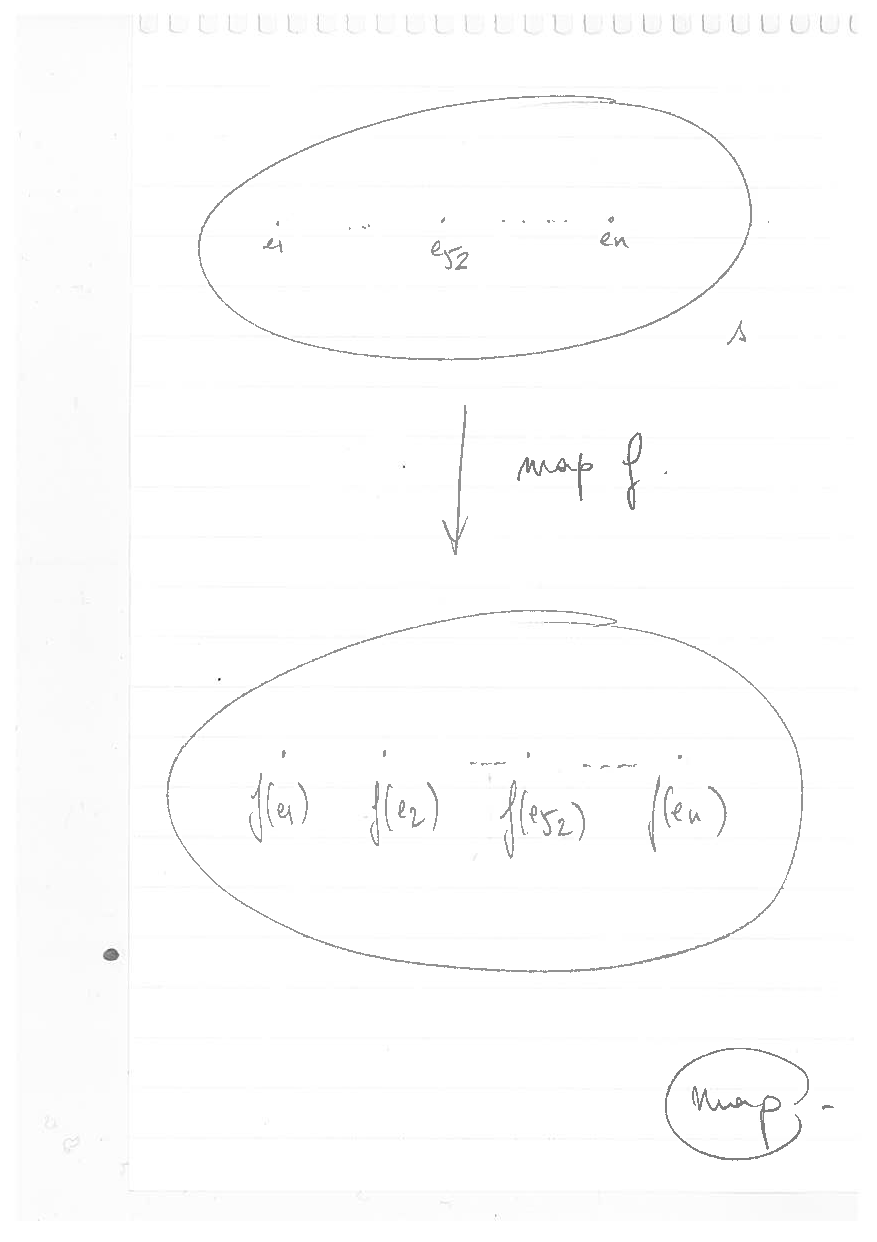
\includegraphics[width=10cm]{map}

The code above uses some new \cat{} constructs: ``\texttt{++}'' is set addition
(in infix notation), ``\verb+{}+ is the empty set.

It also uses set pattern matching that permits recursion over sets,
by considering the empty and non-empty cases, in a manner similar
to list pattern matching.

Then, we generate the set of all possible \cohl{L} for all locations~$L$ as
follows:
\begin{verbatim}
let allCohL = map makeCohL (partitions(M))
\end{verbatim}
%\fixme{jade@Luc: il nous faut des crobards ici}

Now, \texttt{allCohL} is a set of set of relations, each element being the
set of all possible $\cohl{L}$ orders for a specific~$L$.  

We still need to generate all possible unions of the $\cohl{L}$ for
% all possible choices of those\fixme{jade@Luc: c'est qui those ici?} and 
all possible locations~$L$.  It can be done by another \cat{} function:
\texttt{cross}, which takes a set of sets $S = \{S_1, S_2, \ldots, S_n\}$ as
argument and returns all possible unions built by picking elements from each of
the $S_i$: 
%\fixme{jade@Luc: il nous faut des crobards ici}

$$
\left\{\, e_1 \cup e_2 \cup \cdots \cup e_n \mid
e_1 \in S_1, e_2 \in S_2, \ldots, e_n \in S_n \,\right\}
$$

We first define a classical \texttt{fold} function over sets:
given a set $S = \{ e_1, e_2, \ldots, e_n\}$, an initial value~$y_0$
and an associative function $f$~that takes a pair $(e,y)$ as argument,
\texttt{fold} computes:
$$
f (e_{i_1},f (e_{i_2}, \ldots, f(e_{i_n},y_0)))  
$$
where $i_1, i_2, \ldots, i_n$ defines a permutation
of the indices $1, 2, \ldots, n$.

\begin{verbatim}
let fold f =
  let rec fold_rec (es,y) = match es with
  || {} -> y
  || e ++ es -> fold_rec (es,f (e,y))
  end in
  fold_rec
\end{verbatim}
As an example, consider:
\begin{verbatim}
let flatten S = fold (fun (e,y) -> e | y) (S,{})
\end{verbatim}
The function~\verb+flatten+
takes a set of sets as argument and returns their union.
As another example, we could have defined \texttt{map} as follows:
\begin{verbatim}
let map f = fun S -> fold (fun (e,y) -> f S ++ y) (S,{})
\end{verbatim}

We now write \texttt{cross}:
\begin{verbatim}
let rec cross ess = match ess with
  || {} -> { 0 }
  || es ++ ess ->
      let yss = cross ess in
      fold
        (fun (e,r) -> map (fun ys -> e | ys) yss | r)
        (es,{})           
  end      
\end{verbatim}
Notice, in the code above, that we use the union operator ``\verb+|+'' and of
the empty relation ``\verb+0+''. 

Finally we generate all possible $\coh$ ``orders'' by:
\begin{verbatim}
let allCoh = cross allCohL
\end{verbatim}

\subsection{\label{coherence}Coherence}

For a given location~$L$, the coherence order $\cohl{L}$ is defined as a total
order on all loads and stores to location~$L$. The single Coherent Order $\coh$
is the union of all these orders for all locations.  In appendix~\ref{coh} we
describe how to generate the set of all possible $\coh$ orders in the \cat{}
language.  For now, let us assume a variable \texttt{allCoh} whose value is the
set of all possible \coh{} orders.

The instruction \texttt{with $v$ from $S$} will, for each~$e$ in $S$, execute
the rest of the model in an extended environment that binds $v$ to~$e$. For
\coh{}, we write: \verb+with coh from allCoh+. This means that we bind the
variable {\tt coh} to a \coh{} order picked in the set {\tt allCoh}. 

\subsubsection{Consistency of {\tt coh} and {\tt po}}

We can then  check the consistency of $\coh$ and~$\po$:
\begin{verbatim}
call consistent(coh,po) as CohPoCons
\end{verbatim}
See Section~\ref{procedure} for the definition of the consistency check as a
procedure.

%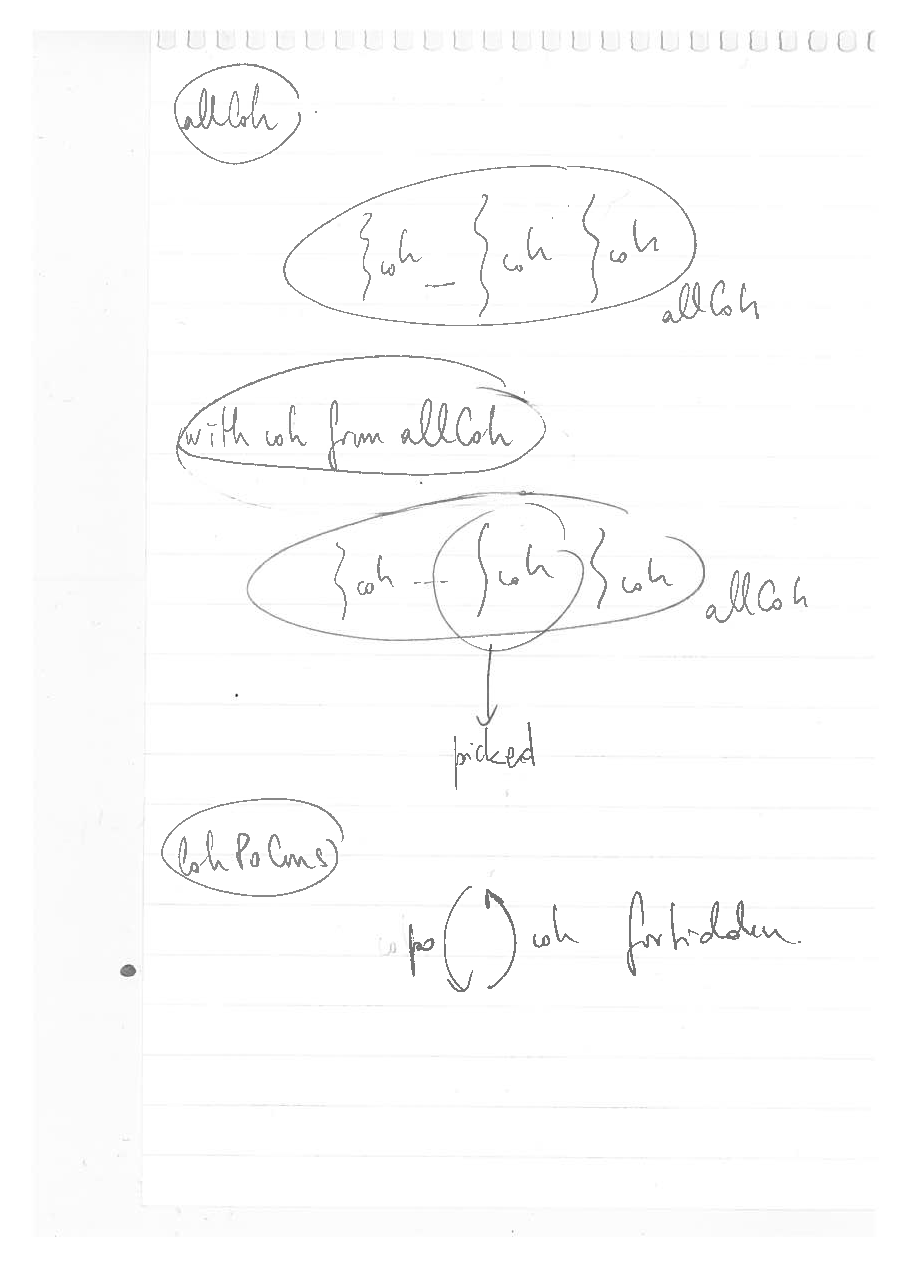
\includegraphics[width=08cm]{allcoh}

\subsubsection{Value of a load}

The ``value of a load'' check states that: ``\emph{a load [\ldots] will always
observe the most recent store in the coherent order of location~$L$}''.

Given a read of location $L$, we find ``the most recent store in the coherent
order of location $L$'' using the relation \texttt{mincohWR}. This relation
is implemented in the \cat{} language as follows:
\begin{verbatim}
let cohWR = coh & (W * R)
let cohWW = coh & (W * W)
let mincohWR = cohWR \ (cohWW; cohWR)
\end{verbatim}
where \verb+W+ is the set of all writes, \verb+R+ the set of all reads,
\verb+W*R+ is the set of write-read pairs (which can also be viewed as a
relation that relates any write to all reads), \verb+W*W+ the set of
write-write pairs, ``\verb+&+'' is intersection, ``\verb+*+'' is cartesian
product and ``\verb+\+'' is (set or relation) difference. To implement ``value
of a load'', we check that $\rf$ equals \texttt{mincohWR}:

\verb+call equals(rf,mincohWR) as LoadCons+

%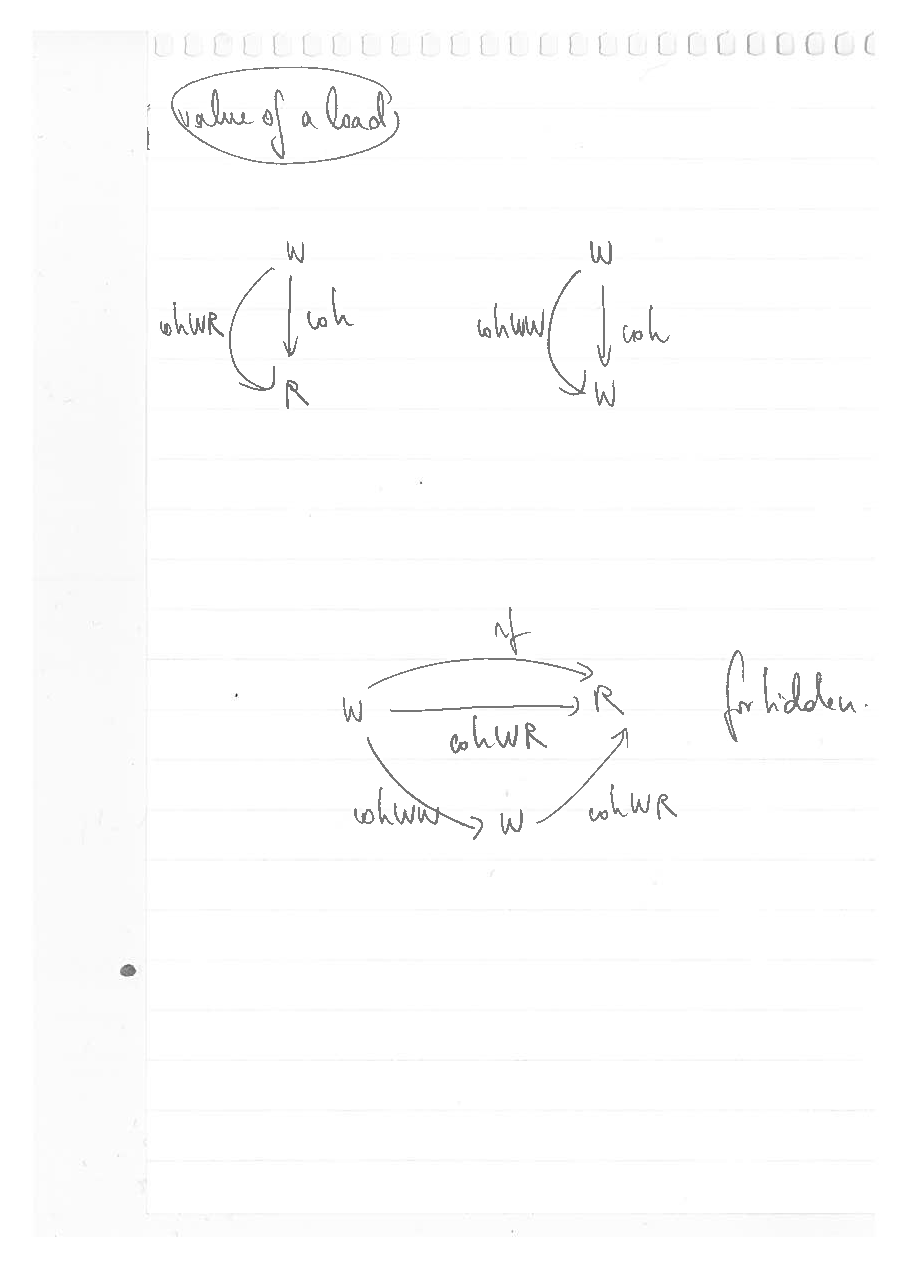
\includegraphics[width=10cm]{value-of-a-load}
%\vspace*{-2mm}
 
See Section~\ref{procedure} for the definition of the procedure {\tt equals}.

\subsubsection{\label{rmw}Read-modify-writes}

A RMW operation corresponds to two events, a read and a write, which are
related by a pre-defined \texttt{rmw} relation.

We state the atomicity of RMW's as follows:
\begin{verbatim}
let cohRW = coh & (R * W)
empty rmw & (cohRW;cohWW) as RmwCons
\end{verbatim}

%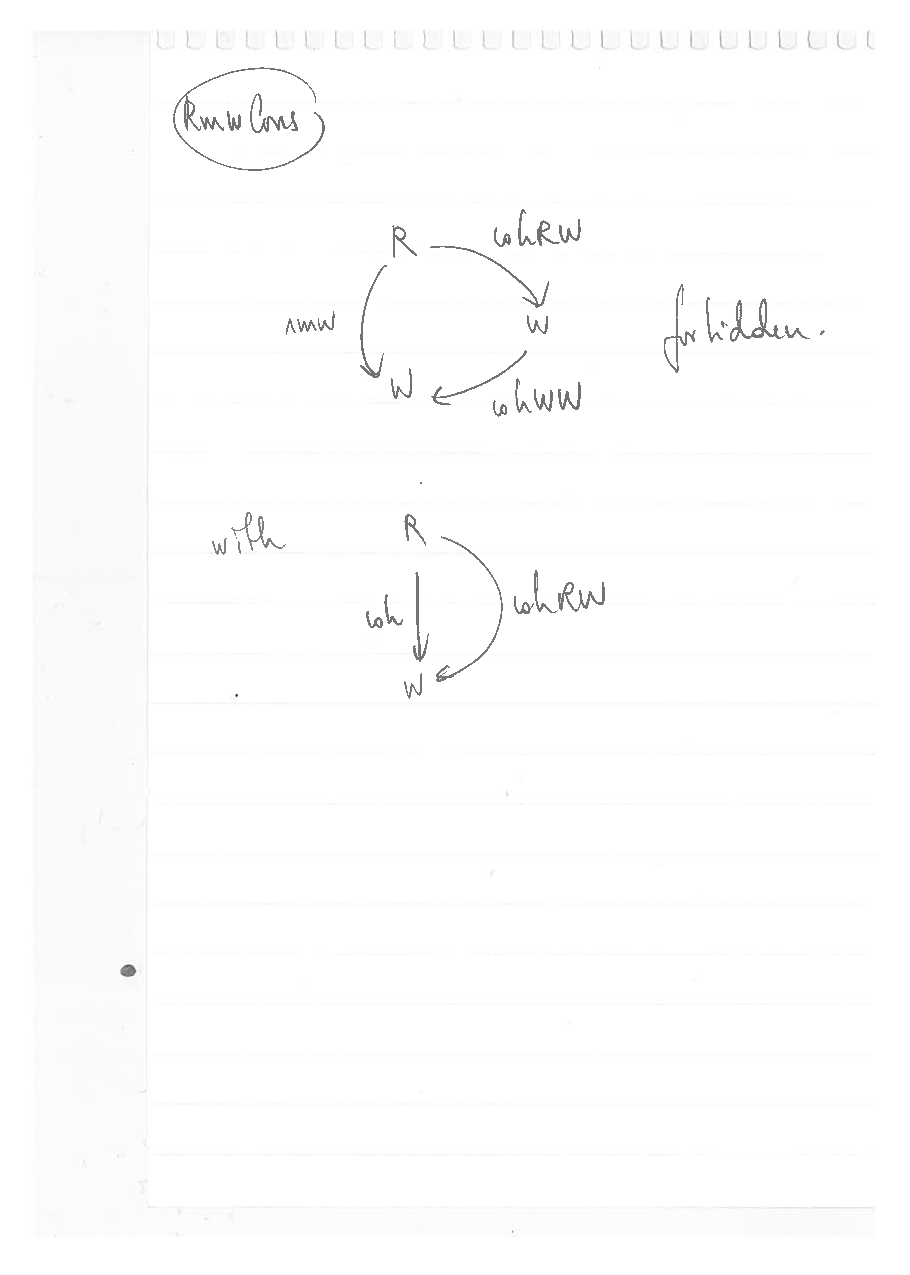
\includegraphics[width=10cm]{rmwcons}

\subsection{Local and global dependence orders}

\subsubsection{Local dependence order}

The document defines the ``local dependence order'' $\ldo$ informally as the
union of data, address and control dependencies (Sec 3.8).

Our \prog{herd} tool provides pre-defined relations for the three kinds of
dependency relations:
Hence we write
\begin{verbatim}
let ldo = data | addr | ctrl
\end{verbatim}

%Note that in the absence of a concrete ISA this essentially amounts to having
%\emph{dependency fences}.

%{\color{blue} We note that no provision is made to restrict control
%dependencies: for example on Power or ARM a branch between two reads does not
%yield a control dependency (one needs to place an {\tt isync} (resp. {\tt isb})
%fence after the branch on Power (resp. on ARM) to create a dependency from read
%to read via a branch).  Is that intentional? Should we restrict {\tt ctrl}?}

\subsubsection{Global dependence order}

The document then defines the ``global dependence order'' as
the irreflexive transitive closure of \ldo{} union \coh{},
which we write
\begin{verbatim}
let gdo = (ldo|coh)+
\end{verbatim}

The document then states
``\emph{By rule, there cannot be a cycle in \gdo{}}'', which we interpret as a
requirement: \gdo{} must be acyclic.

\begin{verbatim}
acyclic gdo as GdoCons
\end{verbatim}

\subsubsection{No thin air}

It seems to us that requiring {\tt gdo} acyclic aims at forbidding \emph{out of
thin air} values, as illustrated by the typical example ``\ltst{lb+ldos}'':
\begin{figure}[!h]
\begin{center}
\moveback\fmt{lb+ldos}
\end{center}
\caption{The load buffering test with {\tt ldos} on both threads
\color{red}{(Forbidden)}}
\end{figure}

See also:
\url{virginia.cs.ucl.ac.uk/?record=hsa&cat=hsa&bell=hsa&litmus=lb+ldos}.
%{\color{blue} We have several questions on that topic:
%\begin{itemize}
%\item Is that right, that the intent is to forbid out of thin air values?
%\item How about placing fences in between the read-write pairs on each
%thread, should that forbid the LB behaviour above?
%\item How about having one step of {\tt ldo} then an internal {\tt coh} step on
%	each thread, should that forbid the LB behaviour? And the other way
%	around? One step of internal {\tt coh} then one step of {\tt ldo} on
%	each thread, should that forbid the LB behaviour?
%\end{itemize}}

% {\color{blue} Let us investigate each of these items in more details:
% 
% \paragraph{Fences}
% 
% Consider this fenced variant of the LB test:
% \begin{verbatim}
% Bell LB+fences 
% {
% x = 0;
% y = 0;
% }
%  P0                              | P1                              ;
%  r[ordinary,rlx,wi,single] r1 x  | r[ordinary,rlx,wi,single] r2 y  ;
%  f[...]                          | f[...]                          ;  
%  w[ordinary,rlx,wi,single] y 1   | w[ordinary,rlx,wi,single] x 1   ;
% 
% scopes:
% (system (agent (wg (wave (wi P0)) (wave (wi P1)))))
% 
% regions: x:global, y:global
% 
% ~exists (0:r1=1 /\ 1:r2=1)
% \end{verbatim}
% 
% Are there any tags we can put on the fences that would forbid the weak
% behaviour of this test (viz the case where both registers hold the value $1$ in
% the end)? We're wondering about both memory order and scope tags. Also, under
% what scope tree or scope instances?
% 
% More generally, should {\tt ldo} include something along the lines of:
% \begin{verbatim}
% (po & (_ * (F & Tag));po) & same-instance('tag)
% \end{verbatim}
% 
% \paragraph{Interaction of {\tt ldo} and {\tt coh}}
% 
% 
% More generally, should {\tt ldo} include something along the lines of:
% \begin{verbatim}
% po-loc 
% \end{verbatim}
% 
% alternatively: 
% \begin{verbatim}
% coh & ~ext
% \end{verbatim}
% 
% For example, consider this variant of the LB test (where {\tt dep} stands for
% ``dependency'', and could be any of {\tt addr, data} or {\tt ctrl}):
% 
% \pagebreak
% 
% \begin{verbatim}
% Bell LB+dep-cohWW+dep
% {
% x = 0;
% y = 0;
% }
%  P0                              | P1                              ;
%  r[ordinary,rlx,wi,single] r1 x  | r[ordinary,rlx,wi,single] r2 y  ;
%  f[dep]                          | f[dep]                          ;  
%  w[ordinary,rlx,wi,single] y 1   | w[ordinary,rlx,wi,single] x 1   ;
%  w[ordinary,rlx,wi,single] y 2   |                                 ;
% scopes:
% (system (agent (wg (wave (wi P0)) (wave (wi P1)))))
% 
% regions: x:global, y:global
% 
% ~exists (0:r1=1 /\ 1:r2=2)
% \end{verbatim}
% 
% Should the weak behaviour of LB be forbidden in this case? Namely the one where
% {\tt r2} on {\tt P1} holds $2$ and {\tt r1} on {\tt P0} holds $1$ at the end.
% 
% Or this variant:
% \begin{verbatim}
% Bell LB+dep-cohRW+dep
% {
% x = 0;
% y = 0;
% }
%  P0                              | P1                              ;
%  r[ordinary,rlx,wi,single] r1 x  | r[ordinary,rlx,wi,single] r2 y  ;
%  f[dep]                          | f[dep]                          ;  
%  r[ordinary,rlx,wi,single] r3 y  | w[ordinary,rlx,wi,single] x 1   ;
%  w[ordinary,rlx,wi,single] y 1   |                                 ;
% scopes:
% (system (agent (wg (wave (wi P0)) (wave (wi P1)))))
% 
% regions: x:global, y:global
% 
% ~exists (0:r1=1 /\ 1:r2=1)
% \end{verbatim}
% 
% Should the weak behaviour of LB be forbidden in this case? Namely the one where
% {\tt r2} on {\tt P1} holds $1$ and {\tt r1} on {\tt P0} holds $1$ at the end.
% 
% \pagebreak
% 
% Or this variant:
% \begin{verbatim}
% Bell LB+dep-cohRW-cohWW+dep
% {
% x = 0;
% y = 0;
% }
%  P0                              | P1                              ;
%  r[ordinary,rlx,wi,single] r1 x  | r[ordinary,rlx,wi,single] r2 y  ;
%  f[dep]                          | f[dep]                          ;  
%  r[ordinary,rlx,wi,single] r3 y  | w[ordinary,rlx,wi,single] x 1   ;
%  w[ordinary,rlx,wi,single] y 1   |                                 ;
%  w[ordinary,rlx,wi,single] y 2   |                                 ;
% scopes:
% (system (agent (wg (wave (wi P0)) (wave (wi P1)))))
% 
% regions: x:global, y:global
% 
% ~exists (0:r1=1 /\ 1:r2=2)
% \end{verbatim}
% 
% Should the weak behaviour of LB be forbidden in this case? Namely the one where
% {\tt r2} on {\tt P1} holds $2$ and {\tt r1} on {\tt P0} holds $1$ at the end.
% 
% Or this variant:
% \begin{verbatim}
% Bell LB+dep-cohRR-dep+dep
% {
% x = 0;
% y = 0;
% }
%  P0                              | P1                              ;
%  r[ordinary,rlx,wi,single] r1 x  | r[ordinary,rlx,wi,single] r2 y  ;
%  f[dep]                          | f[dep]                          ;  
%  r[ordinary,rlx,wi,single] r3 z  | w[ordinary,rlx,wi,single] x 1   ;
%  r[ordinary,rlx,wi,single] r4 z  |                                 ;
%  f[dep]                          |                                 ;  
%  w[ordinary,rlx,wi,single] y 1   |                                 ;
% scopes:
% (system (agent (wg (wave (wi P0)) (wave (wi P1)))))
% 
% regions: x:global, y:global
% 
% ~exists (0:r1=1 /\ 1:r2=1)
% \end{verbatim}
% 
% Should the weak behaviour of LB be forbidden in this case? Namely the one where
% {\tt r2} on {\tt P1} holds $1$ and {\tt r1} on {\tt P0} holds $1$ at the end.
% 
% \pagebreak
% 
% Or this variant:
% \begin{verbatim}
% Bell LB+cohRR-dep+dep
% {
% x = 0;
% y = 0;
% }
%  P0                              | P1                              ;
%  r[ordinary,rlx,wi,single] r1 x  | r[ordinary,rlx,wi,single] r2 y  ;
%  r[ordinary,rlx,wi,single] r3 x  |                                 ;
%  f[dep]                          | f[dep]                          ;  
%  w[ordinary,rlx,wi,single] y 1   | w[ordinary,rlx,wi,single] x 1   ;
% scopes:
% (system (agent (wg (wave (wi P0)) (wave (wi P1)))))
% 
% regions: x:global, y:global
% 
% ~exists (0:r1=1 /\ 1:r2=1)
% \end{verbatim}
% 
% Should the weak behaviour of LB be forbidden in this case? Namely the one where
% {\tt r2} on {\tt P1} holds $1$ and {\tt r1} on {\tt P0} holds $1$ at the end.
% 
% Or this variant:
% \begin{verbatim}
% Bell LB+cohRW-cohWR-dep+dep
% {
% x = 0;
% y = 0;
% }
%  P0                              | P1                              ;
%  r[ordinary,rlx,wi,single] r1 x  | r[ordinary,rlx,wi,single] r2 y  ;
%  w[ordinary,rlx,wi,single] x 1   |                                 ; 
%  r[ordinary,rlx,wi,single] r3 x  |                                 ;
%  f[dep]                          | f[dep]                          ;  
%  w[ordinary,rlx,wi,single] y 1   | w[ordinary,rlx,wi,single] x 1   ;
% scopes:
% (system (agent (wg (wave (wi P0)) (wave (wi P1)))))
% 
% regions: x:global, y:global
% 
% ~exists (0:r1=1 /\ 1:r2=1)
% \end{verbatim}
% 
% Should the weak behaviour of LB be forbidden in this case? Namely the one where
% {\tt r2} on {\tt P1} holds $1$ and {\tt r1} on {\tt P0} holds $1$ at the end.}
% 
%\pagebreak

\subsubsection{Write-to-read causality}

We observe that the definition of {\tt gdo} as is forbids \ltst{wrc+ldos}:

\begin{figure}[!h]
\begin{center}
\moveback\fmt{wrc+ldos}
\end{center}
\caption{The write-to-read causality test with {\tt ldos} \color{red}{(Forbidden)}}
\end{figure}

See also:
\url{virginia.cs.ucl.ac.uk/?record=hsa&cat=hsa&bell=hsa&litmus=wrc+ldos}.
% {\color{blue} Is that intentional? If the intent of requiring {\tt gdo} acyclic
% is only to forbid out of thin air values, then {\tt gdo} could be simplified,
% and only include a fragment of {\tt coh}. More precisely {\tt gdo} could
% include {\tt rfe}, viz the \rf{} relation when source and target belong to
% different units (below the pre-defined relation {\tt ext} gathers pairs of
% events from different units):
% \begin{verbatim} 
% let rfe = rf & ext
% let gdo = (ldo | rfe)+
% acyclic gdo as GdoCons
% \end{verbatim}
% 
% Or even, omitting the transitive closure: {\tt let gdo = ldo | rfe}. Indeed
% taking the transitive closure doesn't change anything when requiring {\tt gdo}
% to be acyclic, and {\tt gdo} is never used later in the model.
% 
% Note (see the event tags in the figure above) that all memory accesses in test
% \ltst{wrc+ldos} are atomic relaxed.  Furthermore, the pictured execution
% validates the coherence constraints (our section~\ref{coherence}) and, provided
% the three units~\myth{0}, \myth{1} and~\myth{2} are in the same work-group, the
% execution is not racy.  Hence, there are no further constraints on this
% execution and the test being allowed or forbidden depends exclusively on the
% definition of \texttt{gdo}.  More precisely with \texttt{gdo} being
% \verb!(ldo|coh)+! the test is forbidden; with \texttt{gdo} being
% \verb!(ldo|rfe)+! the test is allowed.}
% 
% Assuming this is the intent, let us revisit similar questions to the LB ones on
% the WRC test case. 
% 
% \pagebreak
% 
% {\color{blue} Consider the following variant of WRC:
% {\footnotesize
% \begin{verbatim}
% Bell wrc+fence+dep
% {
% 2:r1=-1;
% }
% P0                          | P1                           | P2                           ;
% w[atomic,rlx,wg,single] x 1 | r[atomic,rlx,wg,single] r0 x | r[atomic,rlx,wg,single] r0 y ;
%                             | f[...]                       | bne r0, 1, Exit2             ;
%                             | w[atomic,rlx,wg,single] y 1  | r[atomic,rlx,wg,single] r1 x ;
%                             |                              | Exit2:                       ;
% exists (1:r0=1 /\ 2:r0=1 /\ 2:r1=0)
% \end{verbatim}
% }
% 
% Are there any tags we can put on the fence on {\tt P1} that would forbid the
% weak behaviour of this test (viz the case where on {\tt P1} {\tt r0} holds $1$,
% i.e. {\tt P1} has read from {\tt P0}, and on {\tt P2} {\tt r0} holds $1$, i.e.
% {\tt P2} has read from {\tt P1}, and finally on {\tt P2} {\tt r1} holds $0$,
% meaning {\tt P2} has read $x$ from the initial state)? We're wondering about
% both memory order and scope tags. Also, under what scope tree or scope
% instances?
% 
% And what about this variant:
% {\footnotesize
% \begin{verbatim}
% Bell wrc+dep+fence
% {
% 2:r1=-1;
% }
%  P0                          | P1                           | P2                           ;
%  w[atomic,rlx,wg,single] x 1 | r[atomic,rlx,wg,single] r0 x | r[atomic,rlx,wg,single] r0 y ;
%                              | bne r0, 1, Exit1             | f[...]                       ;
%                              | w[atomic,rlx,wg,single] y 1  | r[atomic,rlx,wg,single] r1 x ;
%                              | Exit1:                       |                              ;
% exists
% (1:r0=1 /\ 2:r0=1 /\ 2:r1=0)
% \end{verbatim}
% }
% 
% Are there any tags we can put on the fence on {\tt P2} that would forbid the
% weak behaviour of this test (viz the case where on {\tt P1} {\tt r0} holds $1$,
% i.e. {\tt P1} has read from {\tt P0}, and on {\tt P2} {\tt r0} holds $1$, i.e.
% {\tt P2} has read from {\tt P1}, and finally on {\tt P2} {\tt r1} holds $0$,
% meaning {\tt P2} has read $x$ from the initial state)? We're wondering about
% both memory order and scope tags. Also, under what scope tree or scope
% instances?}
% 
%\subsubsection{Distributed S shape}
%
%We observe that the definition of {\tt gdo} as is forbids
%\ltst{distributed-S+deps}:
%{\footnotesize
%\begin{verbatim}
%Bell distributed-S+deps
%{
%2:r1=-1;
%}
%P0                          | P1                           | P2                           ;
%w[atomic,rlx,wg,single] x 2 | r[atomic,rlx,wg,single] r0 x | r[atomic,rlx,wg,single] r0 y ;
%                            | f[dep]                       | f[dep]                       ;
%                            | w[atomic,rlx,wg,single] y 1  | w[atomic,rlx,wg,single] x 1  ;
%exists (1:r0=2 /\ 2:r0=1 /\ x=2)
%\end{verbatim}
%}
%
%{\color{blue} Is that intentional? If the intent of requiring {\tt gdo} acyclic
%is only to forbid out of thin air values, then {\tt gdo} could be simplified,
%along the lines of what we write above.}
%

\pagebreak
\subsection{Heterogeneous happens-before}

\subsubsection{Scoped synchronisation order \label{sso}}

We can now define scoped synchronisation orders, which we believe essentially
formalise release-acquire synchronisation, with scope restrictions. 

Recall that \prog{herd} builds pre-defined sets of tagged events; for example
{\tt Screl} is the set of events bearing the tag {\tt screl}. From these sets,
we build a few relevant sets:
\begin{verbatim}
let Release = Screl | Scar
let Acquire = Scacq | Scar
let Synchronizing = Acquire | Release
\end{verbatim}

Note that the \texttt{screl}, \texttt{scacq} and~\texttt{scar} tags apply to
atomic operations and to fences only. As a consequence, the above sets regroup
atomic operations and fences only.

To build the scoped synchronisation order, we follow the documentation (Section
3.9), up to a few minor changes that we detail below:
\begin{verbatim}
let acq-rel =
  (((W | RMW) & Release) * ((R | RMW) & Acquire)) & coh
| ((F & Release) * Acquire) &
  ((po & (_ * (W | RMW))); coh; (po? & ((R | RMW) * _)))
| (Release * (F & Acquire)) &
  ((po? & (_ * (W | RMW))); coh; (po & ((R | RMW) * _)))

let sso(tag) = same-instance(tag) & acq-rel
\end{verbatim}

Note that we do not impose for the intermediate $A$ and~$B$ operations (the
ones such that $A \coh B$) to be atomic accesses in the last two cases.
Although this is a race, we did not find this to be specified in the HSA
document. %{\color{blue} Is that intentional?}

The definition of \texttt{acq-rel} gathers the three top-level items of the
description of the HSA document.  It uses set and relation constructs
intensively, most of which have already been introduced, except the ``optional
step'' operator~\texttt{$e$?} that yields, \texttt{$e$|id} (\emph{i.e.} $e$
union the identity relation), and the universe set ``\verb+_+'' that contains
all events (even fence events).

Our (minor) changes w.r.t. the HSA documentation are:
\begin{itemize}
\item we do not specify the accesses to be synchronising or atomic, as our
\texttt{Acquire} and \texttt{Release} sets contain synchronising
operations~only;
%\item we make no specific provision for
%RMW operations as they are represented by a read event (in~\verb+R+)
%and a write event (in \verb+W+) (see our section~\ref{rmw});
\item we made the definition a bit more symmetric (and redundant) by having the
third item produce fence-to-fence order, as the second item does;

\item we have factored out the condition ``\emph{$X$ and~$Y$ both specify the
same instance~$S$}'' (implemented by the call to ``\verb+same-instance(s)+'').
\end{itemize}

\pagebreak

\paragraph{An example: ISA2}

As an illustration, let us examine the test~\ltst{isa2}:
{\footnotesize
\verbatiminput{img/isa2+coh}
}

Below in Figure~\ref{isa2coh} we consider a particular execution candidate of
the test~\ltst{isa2}, viz a certain~\rf{} relation and a certain~\coh{}
relation:
\begin{figure}[!h]
\begin{center}\fmt{isa2+coh}
\end{center}
\caption{\label{isa2coh}An execution candidate of the test~\ltst{isa2} \color{green}{(Allowed)}}
\end{figure}
%{\color{blue} Does this picture match the intent?}

See also
\url{virginia.cs.ucl.ac.uk/?record=hsa&cat=hsa&bell=hsa&litmus=isa2}.

More precisely,
\begin{itemize}
\item given the condition \verb+exists (1:r0=1 /\ 2:r0=1 /\ 2:r1=0)+ of the
test, we select an execution where the read from~\texttt{y} by the
unit~\myth{1} reads the value \texttt{1}, which is stored to~\texttt{y} by the
unit~\myth{0}.  Hence, we select an execution where $b \rf c$.  Similarily we
select $d \rf e$.  Finally we consider that the event~$f$ reads the initial
value of~\texttt{x}, which is pictured by a red~\rf{} arrow from the
``initial'' event  (top of figure) to event~$f$.

\item We select some \coh{} relation that passes the coherence checks of
section~\ref{coherence}.  For clarity of the picture, we do not show the
complete \coh{} relation but a sub-relation (essentially edges that can be
deduced by transitivity are omitted).  The significant pairs of this \coh{}
relation are $b \coh c$, $d \coh e$ (which are the same as inter-unit \rf{}
pairs), and $f \coh a$ which originates from event~$f$ reading the initial
value of~\texttt{x}, which implies that the event $f$  is \coh-before all
writes to~\texttt{x} performed by all the units of the test.
\end{itemize}

\paragraph{An illustration of sso on ISA2}

Now that we have defined \coh{}, we can compute scope synchronisation orders.
Figure~\ref{isa2sso} shows the scope synchronisation orders for scopes agent
and work-group, for the test ISA2.
\begin{figure}[!h]
\begin{center}\moveback\fmt{isa2+sso}
\end{center}
\caption{\label{isa2sso}Scope synchronisation orders for scopes agent (\textsf{sso-agent}) and work-group (\textsf{sso-wg}) \color{green}{(Allowed)}}
\end{figure}

See also
\url{virginia.cs.ucl.ac.uk/?record=hsa&cat=hsa&bell=hsa&litmus=isa2}.

%{\color{blue} Does this picture match the intent?}
Observe that the pair~$b \sso{wg} c$ results from the first case of the
definition of \verb+acq-rel+, namely 
\verb+((W & Release) * (R & Acquire)) & coh+, 
as $b$ is a write release (tag~\texttt{screl} in Figure~\ref{isa2sso}) and $c$
is a read acquire (tag~\texttt{scacq}).

Furthermore, we have $b \coh c$ (Figure~\ref{isa2coh}), thus the pair~$(b,c)$
is part of \texttt{acq-rel}.  Finally, events $b$ and $c$ specify the same
scope instance of level work-group, as illustrated by the pair $b \same{wg} c$
depicted in Figure~\ref{isa2same}.

Hence,  we have $b \sso{wg} c$, since we defined $\sso{wg}$ as the intersection
of the relations \texttt{acq-rel} and $\same{wg}$ (implemented as
\texttt{same-instance('wg)}).

\subsubsection{Heterogeneous happens-before \label{sec:hhb}}

Following the HSA~document, we define the HSA happens-before order~\hhb{} as
the transitive closure of the union of the program order and of the union of
scope synchronisation order for all scopes:
\begin{verbatim}
let union-scopes f = fold (fun (s,y) -> f s | y) (scopes,{})

let hhb = (po | union-scopes sso)+
\end{verbatim}

The function \texttt{union-scopes} takes a function {\tt f} as argument.  This
function {\tt f} should go from scope tags to relations, typically just like
\texttt{sso}.

The function \texttt{union-scopes} returns the union of the
\texttt{$f(\text{tag})$} for all scope tags.  It refers to the \texttt{scopes}
tag set, which is implicitly defined by the \verb+enum scopes = +\ldots{}
definition, and to the \verb+fold+ (over sets) function, defined in
appendix~\ref{coh}.

In the case of the test~\ltst{isa2} we get the \hhb{} relation pictured
in figure~\ref{isa2hhb}.
\begin{figure}
\begin{center}\fmt{isa2+hhb}
\end{center}
\caption{\label{isa2hhb} The HSA happens-before relation for test~\ltst{isa2} \color{red}{(Forbidden)}}
\end{figure}
Edges that result from the transitivity of~\hhb{} are omitted. In particular
the pair $a \hhb f$ is omitted. 
%{\color{blue} Does this picture match the intent?}

See also: \url{virginia.cs.ucl.ac.uk/?record=hsa&bell=hsa&cat=hsa&litmus=isa2}.

Now, the HSA document defines three validity conditions on~\hhb.  The \hhb{}
relation must be acyclic (equivalently irreflexive, as \hhb{} is transitive),
consistent with \coh{}, and consistent with sequentially consistent orders
(which we shall see in the next section).
We express the first two conditions as follows:
\begin{verbatim}
irreflexive hhb as HhbCons
call consistent (hhb,coh) as HhbCohCons
\end{verbatim}
Note that Figure~\ref{isa2hhb} illustrates a case of inconsistency of \hhb{}
and~\coh{}: $a \hhb f \coh a$. And indeed, our \ltst{isa2} test is
similar to the test ``Race-free transitive synchronisation through multiple
scopes'' of the HSA document (replacing \texttt{while} loops by \texttt{if}
constructs). It should thus be forbidden.

\subsection{Sequentially consistent synchronisation order \label{sc-orders}}
Sec. 3.10 of the HSA document states: ``\emph{there is a total (apparent) order
of all synchronising operations with release, acquire, or acquire-release
semantics in a single scope instance}''.  Given a scope instance~$S$, we write
$\SCS{S}$ for this total order, and $\SCLVL{tag}$ for the union of  $\SCS{S}$
orders for all scope instances at level~\text{tag}. We also abbreviate
sequentially consistent synchronisation order as ``SC order''.

The \cat{} primitive \texttt{classes} takes an equivalence relation as argument
and returns its equivalence classes as a set of sets of events. Hence we can
compute the set of all scope instances~$S$ for a given level~\text{tag}
as follows:
%\marginpar{Luc for Jade, all
%our models use \texttt{same-instance} in place of \texttt{tag2scope}\ldots}

\begin{verbatim}
let sync-instances(tag) =
  classes ((Synchronizing * Synchronizing) & same-instance(tag))
\end{verbatim}
The function~\verb+sync-instance+ takes a scope tag as argument and returns
a set of sets of events, each set of events being a scope instance.

%{\color{blue} Here we could also use {\tt same-instance(lvl)}, which also takes
%into account the scope tags on the synchronisation operations ordered by {\tt
%sync-instances(lvl)}. What is the intent here? Note that choosing {\tt
%tag2scope(lvl)} makes checking the consistency of SC orders wrt one another
%somewhat superfluous, because the domain and range of each SC order are
%included in the domain and range of the wider SC orders, whereas with {\tt
%same-instance} it does not.}

Then, the HSA  document clearly states that the total order $\SC{$S$}$
extends \po{}: ``\emph{Given synchronisation operations $X$ and~$Y$, if $X \po Y$ and $X$ and~$Y$ specify the same scope instance~$S$ (directly or indirectly
through inclusivity), then $X \SC{$S$} Y$}''.
However it is unclear if this applies to any pair of synchronising operations
that belong to~$S$, or only to those whose scope annotations take effect
at the level of~$S$. 
%\fixme{jade: je comprends pas la difference}
%Nevertheless, as $\SC{$S$}$ is total and later required to be consistent
%with $\po$ it does not matter much. 
We choose the first, more simple, interpretation. Hence given a scope
instance~$S$, we compute the set of $\po$ linearisation on~$S$ as follows:
\begin{verbatim}
let preSC = po
let makeSCinstance(S) = linearisations(S,preSC)
\end{verbatim}
The \texttt{linearisation($S$,$r$)} primitive that computes all topological sorts of the graph $(S \times r)$ is introduced in appendix~\ref{coh}.
Finally, we compute the set of all possible $\SCLVL{tag}$ relations as:
\begin{verbatim}
let makeSCscope(tag) = cross (map makeSCinstance (sync-instances(tag)))
\end{verbatim}
The function~\texttt{map} is map over sets. In the code above it serves
to compute the set of the sets of all possible $\SCS{S}$ orders
for all scope instances~$S$ at level~\text{tag}.
The function~\texttt{cross} takes a set of sets $\{S_1,S_2,\ldots,S_n\}$ as
argument and returns its \emph{cross product}, i.e. the set of all sets built
by picking one element in each~$S_i$. Those two functions are introduced in
appendix~\ref{coh}.

%{\color{blue} To help us settle these questions on SC orders, it'd be helpful
%to know whether two synchronising operations by the same unit, bearing the
%annotation work-group should be ordered by the SC order of their scope instance
%of level agent.}

%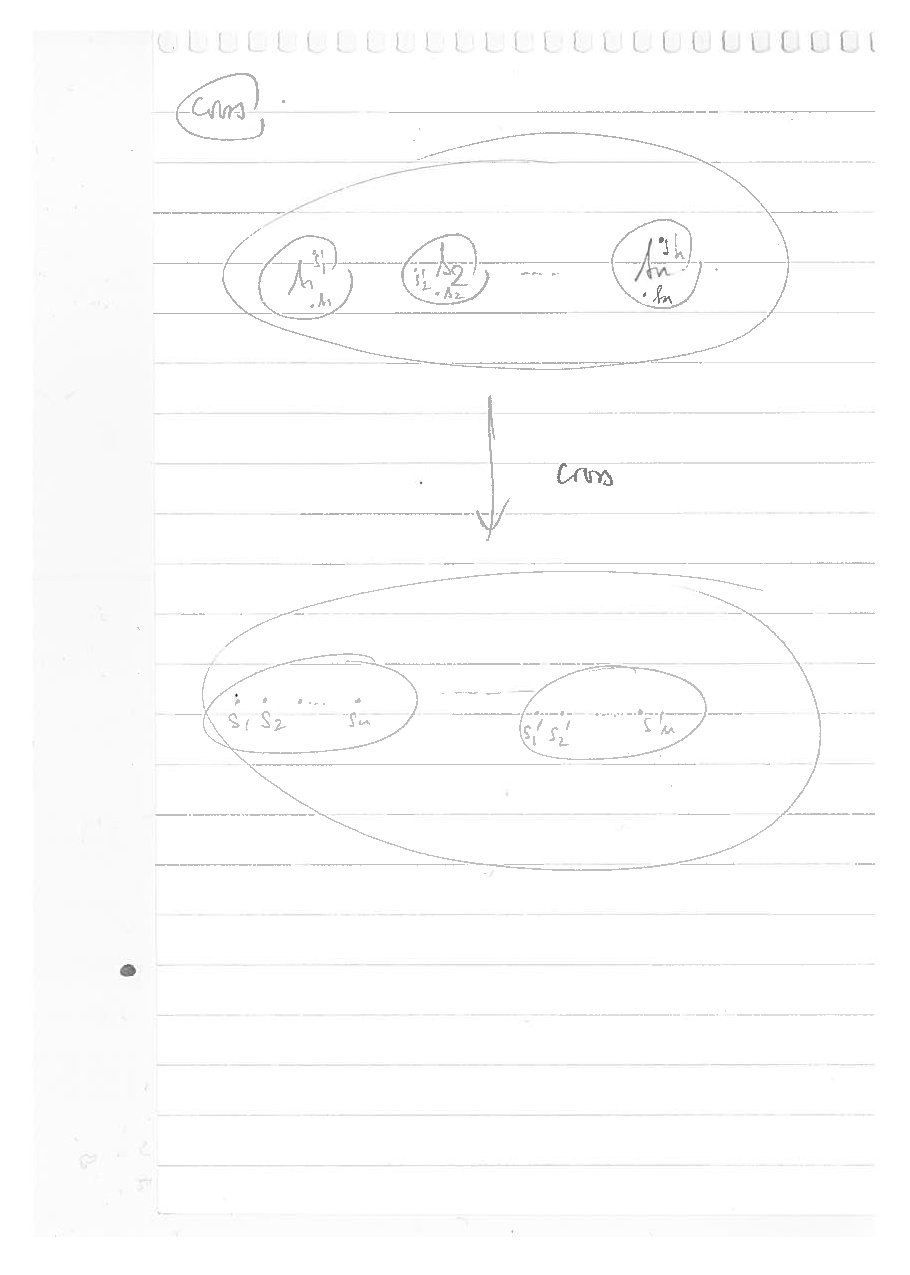
\includegraphics[width=10cm]{cross}

Finally, we iterate over all possible choices of $\SCLVL{tag}$ for the five
HSA scope levels as follows\footnote{A different, more generic,
coding as a loop over the set of scope tags \texttt{scopes} is possible.
We found it to be a bit obfuscated and refrain from presenting it.}: 
%\fixme{jade@Luc: pour la presentation dans ce document, est-ce qu'on pourrait
%mettre tout ca dans une procedure, avec un forall?}
\begin{verbatim}
with SWI from makeSCscope('wi)
call consistent(SWI,coh) as ScCohCons
call consistent(SWI,hhb) as ScHhbCons
with SWAVE from makeSCscope('wave)
call consistent(SWAVE,coh) as ScCohCons
call consistent(SWAVE,hhb) as ScHhbCons
with SWG from makeSCscope('wg)
call consistent(SWG,coh) as ScCohCons
call consistent(SWG,hhb) as ScHhbCons
with SAGENT from makeSCscope('agent)
call consistent(SAGENT,coh) as ScCohCons
call consistent(SAGENT,hhb) as ScHhbCons
with SSYSTEM from makeSCscope('system)
call consistent(SSYSTEM,coh) as ScCohCons
call consistent(SSYSTEM,hhb) as ScHhbCons
\end{verbatim}
Notice that we also check the consistency of SC orders with \coh{} and \hhb{},
as required, but not with~\po{}.  Indeed, by construction the ``order''
\SCLVL{tag} includes~\po{} and the two relations are thus consistent.  It
remains to check that the SC orders are pairwise consistent:
%\marginpar{Luc to Jade, unclear whether omitting the \texttt{ScSc}
%checks will impact valid candidates or not.}
%\fixme{jade@Luc: pour la presentation dans ce document, est-ce qu'on pourrait
%mettre tout ca dans une procedure, avec un forall?}
\begin{verbatim}
call consistent(SWI,SWAVE) as ScSc
call consistent(SWI,SWG) as ScSc
call consistent(SWI,SAGENT) as ScSc
call consistent(SWI,SSYSTEM) as ScSc
call consistent(SWAVE,SWG) as ScSc
call consistent(SWAVE,SAGENT) as ScSc
call consistent(SWAVE,SSYSTEM) as ScSc
call consistent(SWG,SAGENT) as ScSc
call consistent(SWG,SSYSTEM) as ScSc
call consistent(SAGENT,SSYSTEM) as ScSc
\end{verbatim}

\paragraph{An example: SB}

As an example, we consider the following test~\ltst{sb}:
\verbatiminput{img/sb.litmus}
The final proposition \verb+(0:r0 = 0 /\ 1:r0 = 0)+ corresponds
to the \rf{} and \coh{} relations depicted in Figure~\ref{sbcoh}.
\begin{figure}[!h]
\vspace*{-2mm}
\begin{center}\moveback\fmt{sb}
\end{center}
\vspace*{-8mm}
\caption{\label{sbcoh}The non-SC execution of test~\ltst{sb} \color{green}{(Allowed)}}
\end{figure}
See also \url{virginia.cs.ucl.ac.uk/?record=hsa&bell=hsa&cat=hsa&litmus=sb}.

The execution is not sequentially consistent, since there is a cycle in $\po
\cup \coh$. As a result there is no total order that would be consistent with
$\po$ and $\coh$.

The scope tree specification of the test states that the two units of the test
are in the same work group. As a result, all events (which are synchronising
and specify scope work-group) live in the same work-group scope instance.
There is no SC order at the  work-group level. Thus figure~\ref{sbwg} shows a
contradiction between the workgroup SC order SWG and \coh{}.
\begin{figure}[!h]
\vspace*{-2mm}
\begin{center}\moveback\fmt{sb+wg}
\end{center}
\vspace*{-2mm}
\caption{\label{sbwg}Contradiction of the work-group SC order and coh \color{red}{(Forbidden)}}
\end{figure}
See also \url{virginia.cs.ucl.ac.uk/?record=hsa&bell=hsa&cat=hsa&litmus=sb}.

One may observe that the pictured $\SC{wg}$ order contradicts \coh{} on
the pair $(a,d)$.

By contrast, the events of each unit can be ordered independently in each
work-item instance, as show in Figure~\ref{sbwi}.  Indeed the SWI order is
consistent with \po{} (in fact is equal to) and also with \coh{} restricted to
each scope instance, which happen to be empty.
\begin{figure}[!h]
\vspace*{-2mm}
\begin{center}\moveback\fmt{sb+wi}
\end{center}
\vspace*{-2mm}
\caption{\label{sbwi}A successful ordering of the two work-item scope instances \color{green}{(Allowed)}}
\end{figure}
See also \url{virginia.cs.ucl.ac.uk/?record=hsa&bell=hsa&cat=hsa&litmus=sb}.

\pagebreak

\section{Races}
The HSA document has two definitions of conflicts: ordinary and special.
Ordinary conflicts are defined as follows:
``\emph{Two operations $X$ and~$Y$ conflict, iff they access one or
more common byte locations, at least one is a write, and at least one is
an ordinary data operation}''.
Having noticed that ``conflicts'' forms a symmetric relation, we paraphrase
the definition:
\begin{verbatim}
let at-least-one a = (a * _) | (_ * a)

let ordinary-conflicts = loc & at-least-one(W) & at-least-one(Ordinary)
\end{verbatim}
We use the pre-defined relation \verb+loc+ that relates accesses to the same
location, and two pre-defined sets of events: \verb+W+ the set of write
operations, and \verb+Ordinary+ the set of ordinary data operations.

\label{specialconflict}The HSA document defines special conflicts as follows:
\begin{quote}\em
Two special operations $X$ and~$Y$ conflict iff $X$ and $Y$ access
the same byte location and:
\begin{itemize}
\item[35.] $X$ and~$Y$ are different sizes (e.g., 32-bit vs. 64-bit), or
\item[36.] At least one is a write (or a read-modify-write),
and $\neg(\textit{Match}(\textit{SI}(X), \textit{SI}(Y))$.
\end{itemize}
\end{quote}
Condition~36 refers to a (negated) \textit{Match} predicate and to
a~\textit{SI} function.  Both are defined in the ``Scope instances'' section of
the HSA document.

The function~\textit{SI} returns the set of scope instances specified by an
operation, and the \textit{Match} predicate tests the non-emptiness of the
intersection of these scope instances. In Section~\ref{sso} we have defined the
relation~\texttt{same-instance('\text{tag})} that relates events that specify
a common scope instance at level~\text{tag}. Hence, we
represent~\textit{Match} by the relation~\verb+matches+ that relates events
specifying a common scope instance at some level.  In effect, we quantify over
scope levels rather than on pairs of operations and  define \verb+matches+ as
the union of \texttt{same-instance('\text{tag})} for all scope levels. In
\cat{} we write: \begin{verbatim} let matches = union-scopes same-instance

let special-conflicts =
  (loc & (~same-size | Atomic * Atomic) & at-least-one(W)) \ matches
\end{verbatim}
The function~\verb+union-scopes+ that returns the union of
the application of a function on all scope tags is defined
in our Sec.~\ref{sso}. 

The definition of HSA conflicts lacks an additional condition:
accesses have to be by different units, which we consider in
the definition of conflicts below, by the means of the pre-defined~\verb+ext+
relation that relates operations by different units:
\begin{verbatim}
let conflicts = ((ordinary-conflicts|special-conflicts) & ext) \ at-least-one(IW)
\end{verbatim}
We have also added that initial writes (pre-defined set~\verb+IW+)
do not contribute to conflicts.
%As a matter of fact \herd{} considers the initial value of a location to come
%from an explicit initial write operation, for the $\rf$ relation to be defined
%on all read operations.

We then define races as conflicts that are not ordered by HSA happens-before,
in either direction (which we believe to be another omission of the HSA
document):
\begin{verbatim}
let hsa-race = conflicts \ (hhb | hhb^-1)
\end{verbatim}
We used the postfix~$r\texttt{\^{}-1}$ operator that evaluates to
the inverse of relation~$r$.

We inform the \prog{herd} tool about races using with the \texttt{flag}
construct, which apply to all checks.  The normal behaviour for a check is to
stop model execution when invalid.  By contrast, a failing flagged check does
not stop execution but instead ``flags'' it with an arbitrary flag (here
\verb+undefined+).

Flags are recorded and handed over to the \prog{herd} machinery at the end of
model execution --- hence for valid executions that passed all (unflagged)
checks.  The \prog{herd} tool can then decide that the simulated program is
undefined, as soon as one of the valid executions has been flagged as
\verb+undefined+.
\begin{verbatim}
flag ~empty hsa-race as undefined
\end{verbatim}
Observe that the execution is flagged when the \verb+hsa-race+ relation is
\emph{not} empty.

\pagebreak

\section{Cat file}

We gather all the definitions over relations and orders in a {\tt cat} file,
which we give below.

We first give util definitions, e.g. {\tt map} or {\tt fold}, gathered in the file {\tt hsa-lib.cat}:
\verbatiminput{hsa-lib.cat}

\pagebreak

Then the main body of the model ({\tt hsa.cat}):
\verbatiminput{hsa.cat}

\pagebreak

And then the definitions relative to races ({\tt hsa-race.cat}):
\verbatiminput{hsa-race.cat}


\pagebreak

\section{Tests from the documentation}

Here we gather the examples given in the documentation, together with a picture
of a forbidden execution, and a link to the web interface of the {\sf herd}
simulator of our HSA model.

\subsection{Synchronizing operations are sequentially consistent by definition}
\begin{multicols}{2}
\verbatiminput{img/HSA01.litmus}
\end{multicols}
\begin{figure}[htp]
\begin{center}\moveback\fmt{HSA01}
\end{center}
\caption{\label{hsa01} \ltst{HSA01} is forbidden by the consistency
of \SC{wg} and \coh{} \color{red}{(Forbidden)}}
\end{figure}

On the web:

\url{http://virginia.cs.ucl.ac.uk/herd/?record=hsa&bell=hsa&cat=hsa&litmus=HSA01}

\pagebreak

\subsection{Synchronization between units of execution}
\verbatiminput{img/HSA02.litmus}

\begin{figure}[htp]
\begin{center}\moveback\fmt{HSA02}
\end{center}
\caption{\label{hsa02} \ltst{HSA02} is forbidden by the consistency
of \hhb{} and \coh{} \color{red}{(Forbidden)}}
\end{figure}

On the web:

\url{http://virginia.cs.ucl.ac.uk/herd/?record=hsa&bell=hsa&cat=hsa&litmus=HSA02}

\pagebreak

\subsection{Transitivity with a single scope}
\verbatiminput{img/HSA03.litmus}

\begin{figure}[H]
\begin{center}\moveback\fmt{HSA03}
\end{center}
\caption{\label{hsa03} \ltst{HSA03} is forbidden by the consistency
of \hhb{} and \coh{} \color{red}{(Forbidden)}}
\end{figure}

On the web:

\url{http://virginia.cs.ucl.ac.uk/herd/?record=hsa&bell=hsa&cat=hsa&litmus=HSA03}

\pagebreak

\subsection{\label{ex04}Synchronization through multiple scopes}
\verbatiminput{img/HSA04.litmus}
%{\color{blue}
%In the HSA document, all variables, including
%the variable~\texttt{z},
%are defined in the group segment. However
%the variable~\texttt{z} is used ti
%synchronize \myth{1} and~\myth{2}, which are not in the same work-group.
%This looks like a minor error.
%\noindent\textbf{NB:} As segments are not implemented yet
%in \herd{}, we assume global segment for all variables.}

\begin{figure}[htp]
\begin{center}\moveback\fmt{HSA04}
\end{center}
\caption{\label{hsa04} \ltst{HSA04} is forbidden by the consistency
of \hhb{} and \coh{} \color{red}{(Forbidden)}}
\end{figure}

On the web:

\url{http://virginia.cs.ucl.ac.uk/herd/?record=hsa&bell=hsa&cat=hsa&litmus=HSA04}

\pagebreak

\subsection{Synchronization through scope inclusion}
\verbatiminput{img/HSA05.litmus}

\begin{figure}[htp]
\begin{center}\moveback\fmt{HSA05}
\end{center}
\caption{\label{hsa05} \ltst{HSA05} is forbidden by the consistency
of \hhb{} and \coh{} \color{red}{(Forbidden)}}
\end{figure}

On the web:

\url{http://virginia.cs.ucl.ac.uk/herd/?record=hsa&bell=hsa&cat=hsa&litmus=HSA05}

\pagebreak

\subsection{Synchronization through scope inclusion and scope transitivity}
\verbatiminput{img/HSA06.litmus}
This example is quite similar to~\ltst{HSA04} (see Section~\ref{ex04}).
There are two differences:
\begin{itemize}
\item All variables of test~\ltst{HSA06} are in the global segments,
while they are in the group segment in example~\ltst{HSA04}
\item The
scope annotations of the read acquire operation on variable~\texttt{y} by
unit~\myth{1} (event~$c$ in figures~\ref{hsa04} and~\ref{hsa06}) differ:
 it is agent for~\ltst{HSA06} and work-group for~\ltst{HSA04}.
In that sense, this test~\ltst{HSA06} looks like
a combination of the two previous tests~\ltst{HSA04} and~\ltst{HSA05}.
\end{itemize}

\begin{figure}[htp]
\begin{center}\moveback\fmt{HSA06}
\end{center}
\caption{\label{hsa06} \ltst{HSA06} is forbidden by the consistency
of \hhb{} and \coh{} \color{red}{(Forbidden)}}
\end{figure}

On the web:

\url{http://virginia.cs.ucl.ac.uk/herd/?record=hsa&bell=hsa&cat=hsa&litmus=HSA06}

\pagebreak


\subsection{Coh and hhb must be consistent}

\verbatiminput{img/HSA07.litmus}
As expected the test~\ltst{HSA07} is forbidden by the consistency of \hhb{}
and~\coh (see Figure~\ref{hsa07}).  We observe that all the previous tests,
except~\ltst{HSA01}, illustrate the consistency of \hhb{} and~\coh{}.

On the web:

\url{http://virginia.cs.ucl.ac.uk/herd/?record=hsa&bell=hsa&cat=hsa&litmus=HSA07}

\begin{figure}[htp]
\caption{Test~\ltst{HSA07} is {\color{red}{forbidden}} by\ldots}
\begin{center}
\subfloat[\label{hsa07} \ldots{} the consistency of \hhb{}
and~\coh{}.]{\rule{2cm}{0cm}\fmt{HSA07}
\rule{2cm}{0cm}}

\vspace*{2cm}

\subfloat[\label{hsa07bis} \ldots or by value of a load.]{\fmt{HSA07+BIS}}
\end{center}
\end{figure}

One may remark that forbidding this test also results
from the value-of-a-load rule. Figure~\ref{hsa07bis} illustrate this point:
here the relations~\hhb{} and~\coh{} are consistent.
Yet the arrow $a \rf e$ violates value-of-a-load,
as the read~$e$ does not get its value from the most recent write in~\coh{}.

\pagebreak

%\subsection{Separate segment synchronization}
%{\color{blue} From our perspective there is a problem with this example. The
%HSA document comments ``The example shows that synchronisation can cross
%segments. Even though the atomic stores and loads specify a location in global
%memory, they still synchronise the group location~Y''. However the atomic
%stores and loads specify location~Y, which belongs to the group segment.
%Moreover, we still do not quite understand how memory segments fit in the
%memory model. See our remarks in Section~\ref{segment}.}
%\pagebreak

\subsection{Synchronization between units of execution using relaxed atomics}
\verbatiminput{img/HSA09.litmus}

This test illustrates successful synchronization by the means of fences (see
Figure~\ref{hsa09}).  It should perhaps be noted that in this scenarion, fences
are enough to restore~SC.  This would not be the case for test~\ltst{HSA12}
(Section~\ref{ex12}).

\begin{figure}[htp]
\begin{center}\moveback\fmt{HSA09}
\end{center}
\caption{\label{hsa09} \ltst{HSA09} is forbidden by the consistency
of \hhb{} and \coh{} \color{red}{(Forbidden)}}
\end{figure}

On the web:
\url{http://virginia.cs.ucl.ac.uk/herd/?record=hsa&bell=hsa&cat=hsa&litmus=HSA09}

\pagebreak

\subsection{Store speculation is not observable}
\verbatiminput{img/HSA10.litmus}

\begin{figure}[htp]
\begin{center}\moveback\fmt{HSA10}
\end{center}
\caption{\label{hsa10} \ltst{HSA10} is {\color{red}{forbidden}} by the
irreflexivity of~$\gdo{} = (\ldo \cup \rfe)^{+}$}
\end{figure}

On the web:
\url{http://virginia.cs.ucl.ac.uk/herd/?record=hsa&bell=hsa&cat=hsa&litmus=HSA10}

\pagebreak

\subsection{~No out-of-thin-air values}

\verbatiminput{img/HSA11.litmus}
This is the paradigmatic ``no values out-of-thin-air'' test.
As illustrated by Figure~\ref{hsa11}, our models reject this
tests by the irreflexivity check of~\gdo{}.
Observe that the value of events is a variable ``\textsf{S4}''.
This variable stands for just any integer value.

\begin{figure}[htp]
\begin{center}\moveback\fmt{HSA11}
\end{center}
\caption{\label{hsa11} Test~\ltst{HSA11} is {\color{red}{forbidden}} by the
irreflexivity of~$\gdo{} = (\ldo \cup \rfe)^{+}$}
\end{figure}

On the web:
\url{http://virginia.cs.ucl.ac.uk/herd/?record=hsa&bell=hsa&cat=hsa&litmus=HSA11}

\pagebreak

\subsection{\label{ex12}~Dekker's Algorithm}

\verbatiminput{img/HSA12.litmus}

\begin{figure}[htp]
\begin{center}\moveback\fmt{HSA12}
\end{center}
\caption{\label{hsa12} Test~\ltst{HSA12} is \color{green}{allowed}}
\end{figure}

On the web:
\url{http://virginia.cs.ucl.ac.uk/herd/?record=hsa&bell=hsa&cat=hsa&litmus=HSA12}

\begin{figure}[htp]
\begin{center}\moveback\fmt{HSA12+fences}
\end{center}
\caption{\label{hsa12fences} Test~\ltst{HSA12+fences} is \color{green}{allowed}}
\end{figure}

On the web:
\url{http://virginia.cs.ucl.ac.uk/herd/?record=hsa&bell=hsa&cat=hsa&litmus=HSA12+fences}

\pagebreak

\subsection{~Conflict without synchronization}
\verbatiminput{img/HSA13.litmus}
This test illustrates an ordinary race.
There is no \hhb-induced order between events $a$ and~$b$, which
are to the same location, by different units, one event ($a$) being a write,
see~Figure~\ref{hsa13}.
\begin{figure}[htp]
\begin{center}\moveback\fmt{HSA13}
\end{center}
\caption{\label{hsa13} Test~\ltst{HSA13} is racy \color{blue}{(Racy)}}
\end{figure}

On the web:
\url{http://virginia.cs.ucl.ac.uk/herd/?record=hsa&bell=hsa&cat=hsa&litmus=HSA13}

\pagebreak

\subsection{~Insufficient scope}
\verbatiminput{img/HSA14.litmus}
This test illustrates a special race due to non-matching scopes.
Figure~\ref{hsa14} depicts two races: one is between atomic events~$b$ and~$c$
and stems from $b$ and~$c$ belonging to different work-groups, while bearing
the \texttt{wg} scope annotation.  More precisely, Figure~\ref{hsa14bis}
depicts the relations~\same{wg} and~\symr{matches}, which do \emph{not} relate
$b$ and~$c$.  And indeed, (see Section~\ref{specialconflict}) pairs related by
\symr{matches} are subtracted from potential special races.

Moreover, as a result of $b$ and~$c$ being in different work-groups,
the events $a$ and~$d$ are not ordered by \hhb (which reduces to~\po),
and we have a second (ordinary) race.
\begin{figure}[htp]
\begin{center}
\subfloat[\label{hsa14} Test~\ltst{HSA14} is racy.]{\fmt{HSA14}\rule{2cm}{0cm}}

\subfloat[\label{hsa14bis} Scopes for test~\ltst{HSA14}.]{\fmt{HSA14+SCOPE}}
\end{center}
\caption{Test~\ltst{HSA14} is \color{blue}{racy}}
\end{figure}

On the web:
\url{http://virginia.cs.ucl.ac.uk/herd/?record=hsa&bell=hsa&cat=hsa&litmus=HSA14}

%\section{Examples}

Here we show additional examples. 
%The first $5$ ones are classical ones that we
%feel are worth mentioning. 
They are slightly more involved scenarios coming from discussions with the HSA
committee.

%\subsection{SC per location}

%\begin{figure}[htp]
%\caption{\label{hsa13} Test~\ltst{coWW} is forbidden.}
%\begin{center}\moveback\fmt{coww}
%\end{center}
%\end{figure}

%\subsection{Tony1}

%Tony proposed the following scenario:
%\begin{quotation}
%o   Assuming work-items release to agent scope when complete:
%
%�  dispatch work items could do an atomic\_st\_screl\_agent to hidden variable
%provided by packet processor
%
%�         probably do a rmw to a single counter
%
%�  packet processor does atomic\_ld\_acq\_agent on that variable so gets all data
%written by dispatch
%
%�         probably spin until counter to wait for whole dispatch to complete
%
%�  packet processor would do memfence\_screl\_system if indicated by packet release fence
%
%�  packet processor then does an atomic\_st\_rlx\_system to completion signal
%
%�  host (or other) thread does atomic\_ld\_rlx\_system on completion signal
%
%�  host (or other) thread can do a memfence\_scacq\_system if want to access generated data of dispatch
%
%o   Does this model result in correct semantics given current memory model?
%\end{quotation}

%\begin{figure}[!h]
%\setlength{\columnseprule}{.5pt}
%\begin{multicols}{2}
%\small
%\verbatiminput{img/t1-alt.litmus}
%\end{multicols}
%\caption{A tentative packet processor fence scenario\label{ppf}}
%\end{figure}
%{\color{blue} We implement it as shown in Figure~\ref{ppf}.  First, does the
%test match the intent? 
%This test implements the following scenario: \myth{0}
%sends the value $1$ to \myth{1} via $x$ and to \myth{2} via $y$. Then both {\tt
%P1} and {\tt P2} make calculations over $x$ and $y$ respectively, then
%increment the counter $c$ atomically. When the counter has reached $2$,
%\myth{0} accesses $x$ and $y$, and writes their updated values in the variables
%{\tt d1} and {\tt d2}. After doing a release fence at system scope, \myth{0}
%then sends a signal to \myth{3} via variable $s$; \myth{3} can then read {\tt
%d1} and {\tt d2} after having done an acquire fence at system scope.
%
%Our tool produces the same outcomes on the SC and HSA models, which means that
%this test should have enough synchronisation to behave as on SC.  The figures
%\ref{t100} and~\ref{t101} depict the two SC executions where \myth{3} reads the
%value~$1$ from the flag variable~\texttt{s}.  The two executions only differ by
%the order in which \myth{1} and \myth{2} increment the counter \texttt{c}.

%\begin{figure}
%\caption{\label{t100}First execution of test~\ltst{Tony1}}
%\begin{center}
%%\moveback\fmt{t1-00}
%\end{center}
%\end{figure}

%\begin{figure}
%\caption{\label{t101}Second execution of test~\ltst{Tony1}}
%\begin{center}
%%\moveback\fmt{t1-01}
%\end{center}
%\end{figure}
%\pagebreak

\subsection{Tony2}

Here we examine another test:
%proposed by Tony, from a question raised by Hakan:

{\footnotesize
\verbatiminput{img/t2.litmus}
}

The test condition \verb+(2:r2=0 \/ 2:r3=0)+ groups three possible test
outcomes: one of the register being zero and not the other, and both register
being zero.
%We first depict a candidate execution where both
%register hold a final value of zero.
%\begin{figure}
%\caption{\label{t2fig}One execution of test~\ltst{Tony2}}
%\begin{center}\moveback\fmt{t2}\end{center}
%\end{figure}
The test performs two release-acquire synchronisations and thus
resembles the test~\ltst{isa2} (Figure~\ref{isa2coh}),
with the following differences:
\begin{itemize}
\item Two variables (\texttt{x} and~\texttt{y}) are synchronised
where~\ltst{isa2} synchronised only one variable.
\item There is a fence on~\myth{0}, but it does not seem to contribute to
synchronisation, because deleting the fence does not change test behaviour on
our model.
\item The scope tree is different.  More precisely the test~\ltst{Tony2} has
two work-groups scope instances $\{\myth{0}, \myth{2}\}$ and $\{\myth{1}\}$.
That is, \myth{0} and~\myth{2} synchronise through a unit (\myth{1}) that is
not a member of their work-group. Nevertheless, all units belong to the same
agent, and all synchronising actions (events $c$, $d$, $e$ and~$f$) bear the
\texttt{agent} scope tag.
\end{itemize}
As a result, there are happens-before edges from the writes $a$ (to~\texttt{x})
and~$b$ (to \texttt{y}) by \myth{0} to the reads of the same locations
by~\myth{2} (namely $g$ and~$h$). This suffices to forbid the specified
executions as there is a contradiction with~\coh{}.

For analysing how the test is forbidden in detail we relax some checks,
\emph{i.e.} we run the model without performing some checks.  First, by
relaxing the consistency of $\hhb$ and $\coh$ (i.e. calling \prog{herd} with
option \texttt{-skipchecks HhbCohCons}), we get one extra outcome: 
\verb+2:r2=1 /\ 2:r3=0+. The corresponding execution is shown in Figure~\ref{t2hhb}.

\begin{figure}[H]
\caption{\label{t2hhb}Relaxing the consistency of \hhb{} and \coh{}}
\begin{center}\moveback
\fmt{t2+hhb}
\end{center}
\end{figure}
In other words, the location~\texttt{x}, which is accessed by ordinary load and
store instructions is synchronised solely by the means of the consistency of
\hhb{} and \coh{}.  The figure clearly shows the inconsistency:
$a \hhb h \coh a$.
It is important to note that relaxing the consistency of
$\hhb$ and~$\coh$ does not change $\hhb$,
although \hhb{} is defined in terms of a sub-relation~of~$\coh$.

However, event~$g$ still cannot read zero, or, equivalently,
register \verb+2:r2+ cannot contain zero at the end of execution.
This means that the behaviour is
still rejected by other checks of the model.  As a matter of fact all accesses
to location~\texttt{y} are atomic and even synchronising. 

We thus examine sequentially consistent orders. We first assume that, for a
given scope instance~$S$ the SC order $\SCS$ orders all synchronising events
in~$S$, regardless of their scope annotations (i.e. we formalise {\tt
sync-instances} using {\tt tag2scope}, see discussion in Section
\ref{sc-orders}).  It is then enough to relax the consistency of SC orders and
\coh{} to observe a value of zero for the read~$g$.
\begin{figure}[htp]
\caption{\label{t2agent}Relaxing further the consistency of SC orders and of~\coh{}}
\begin{center}\moveback
\fmt{t2+agent}
\end{center}
\end{figure}
The contradiction is visible on Figure~\ref{t2agent}: $b \SC{agent} g \coh b$.
Note that $b \SC{agent} g$ stems from the consistency of SC orders and~\hhb.

We now consider an alternative definition of the domain of
SC orders:  $\SCLVL{tag}$ now operates
on events that specify the scope~\text{tag} (or higher),
\emph{i.e.} we consider event scope annotations.
Such a restricted ``scope instance''
is depicted in figure~\ref{t2scope} as the equivalence relation
$\same{agent}$.
\begin{figure}[htp]
\caption{\label{t2scope}Restricted scope instance of level agent}
\begin{center}\moveback
\fmt{t2+scope}
\end{center}
\end{figure}
Note that neither~$b$ (write to~\texttt{y} by~\myth{0}) nor~$g$ (read
from~\texttt{y} by~\myth{2}) are part of the domain of~\SC{agent}. Thus
preventing $g$ from reading zero (\emph{i.e.} $g \coh b$) cannot come from a
contradiction between $\coh$ and~$\SC{agent}$.

The behaviour becomes allowed if we relax the consistency of SC orders and HSA
happens-before with $\coh$.  To understand how, note that the events $b$
and~$g$ are in the same work-group scope instance, and have the appropriate
\texttt{wg} scope tag.  Hence $b$ and~$g$ must be ordered by $\SC{wg}$, and, as
illustrated by Figure~\ref{t2wg}, the order must be $b \SC{wg} g$, which leads
to the sought contradiction with~\coh{}.

\begin{figure}[htp]
\caption{\label{t2wg}Relaxing further the consistency of SC orders and~\coh{}}
\vspace*{-5mm}
\begin{center}\moveback\fmt{t2+wg}
\end{center}
\vspace*{-5mm}
\end{figure}
Note that $b \SC{wg} g$ stems from $b \hhb g$ by consistency of $\SC{wg}$
and~\hhb.

\subsection{Tony3}
The following test has the same scope tree as the previous~\ltst{Tony2},
\emph{i.e.} there are two work-groups, $\{\myth{0}, \myth{2}\}$
and~$\{\myth{1}\}$; and one agent $\{\myth{0}, \myth{1}, \myth{2}\}$.  It has
no significant~\hhb{} relation as there are no \rf{}~in the execution of
interest.

{\footnotesize
\verbatiminput{img/t3.litmus}
}

This test is forbidden by our models. This is rather comforting as the test is
not sequentially consistent ($\po \cup \coh$ has a cycle), and that using
synchronising stores and loads should restore sequential consistency.
%{\color{blue} (is that the intent?).}

However, restoring SC with synchronising accesses becomes a bit subtle in the
presence of several scope instances.

First, we examine our test under our first option for defining the domain of SC
orders, \emph{i.e.} we consider that a given SC order is defined over all the
synchronising events emitted by the units in a given scope instance (option
{\tt tag2scope} in the definition of {\tt sync-instance}, see
Section~\ref{sc-orders}). As for~\ltst{Tony2} our model rejects the test by the consistency of~\SC{agent}
(defined over all events here) and~\coh{}.  Figure~\ref{t3fst} shows such a
contradiction.

\begin{figure}[h!]
\caption{\label{t3fst}Relaxing the consistency of SC orders
and~\coh{} for the test~\ltst{Tony3}}
\vspace*{-5mm}
\begin{center}\moveback\fmt{t3+fst}
\end{center}
\vspace*{-5mm}
\end{figure}

Then, we consider our second option for SC orders, \emph{i.e.} we consider that
a given SC order is defined over the events that specify a given scope instance
(option {\tt same-instance} in the definition of {\tt sync-instance}, see
Section~\ref{sc-orders}).

\begin{figure}[h!]
\caption{\label{t3}Relaxing the pairwise consistency of SC order for test~\ltst{Tony3}}
\vspace*{-5mm}
\begin{center}\moveback\fmt{t3}
\end{center}
\vspace*{-5mm}
\end{figure}
Figure~\ref{t3} illustrates that the pairwise consistency of SC orders is
instrumental in forbidding the test.  Namely, by the consistency of SC order
with \po{} and~\coh, we have $b \SC{agent} e$ (all intermediate events are in
the same agent scope instance and bear appropriate scope annotations);
similarly we have $e \SC{wg} b$, and thus reach an inconsistency.





\bibliographystyle{plain} \bibliography{hsa}

\end{document}


